\addtocontents{toc}{\setcounter{tocdepth}{3}}
\addtocontents{toc}{\setcounter{tocdepth}{\defaulttocdepth}}

\chapter{Early Season}

\section{Design}
This section documents the proposed design solutions for the VURC ``Push Back'' challenge. We analyze well-known mechanisms, highlight their strengths and weaknesses, and define the architecture for our two robots. This chapter will be split into a total of three overall sections \textbf{Design}, \textbf{Production}, and \textbf{Logs.} From this, we will be able to effectivity explain any brainstorming from the beginning of the design to the final product.
\newline 

\subsection{Design Philosophy}
As a VURC team, we operate under the freedoms of Appendix C, specifically rule \textbf{$<$VUR4$>$}, which permits the manufacturing of parts from legal raw stock.

\begin{figure}[H]
    \centering
    \includegraphics[width=0.95\textwidth]{images/Rules/VURC 4.png}
    \caption{Rule $<$VUR4$>$ Definition: Raw Stock Allowances}
    \label{fig:vur4_rule}
\end{figure}

\textbf{Hybrid Approach:}
For the initial design phase, we have elected to utilize standard VEX parts and rather than designing our own. Using off-the-shelf components allows for rapid prototyping and iteration. However, for structural components where standard parts fail to meet our packaging needs (such as the drivetrain side plates), we will utilize our CNC and 3D printing capabilities to fabricate custom solutions.
\newline

\section{Strategic Architecture: Two 15'' Robots}
This year, Team ATUM has decided to design \textbf{one optimized 15'' robot} and clone it.
\\ \textbf{Reasoning:}
\begin{enumerate}
    \item \textbf{Resource Concentration:} Instead of splitting our engineering hours between two different chassis designs, we can dedicate 100\% of our R\&D time to perfecting a single machine.
    \item \textbf{Maintenance:} In previous years, maintaining two distinct robots caused logistical friction. Identical robots allow for a unified spare parts inventory.
    \item \textbf{Field Consistency:} Drivers can switch between robots without relearning muscle memory.
\end{enumerate}


\subsection{Drivetrain Brainstorming}
Having identified the game challenge, the drivetrain is the most critical subsystem. Considering the constraint of the 15'' limit and the need for high traction, we evaluated four common drivetrain topologies.

% The Decision Matrix Table
\begin{table}[H]
    \centering
    \caption{Drivetrain Decision Matrix (1 = Low, 4 = High)}
    \label{tab:drive_matrix}
    \begin{tabular}{lcccc}
        \toprule
        \textbf{Drive Type} & \textbf{Speed Multiplier} & \textbf{Torque} & \textbf{Simplicity} & \textbf{Strafing} \\
        \midrule
        Tank Drive & 1.0 & High & 4 & No \\
        X-Drive & 1.4 & Low (0.7) & 1 & Yes \\
        H-Drive & 1.0 & Med & 2 & Yes \\
        Mecanum & 1.0 & Med & 3 & Yes \\
        \bottomrule
    \end{tabular}
\end{table}

\textbf{Analysis:}
\begin{itemize}
    \item \textbf{Speed:} The X-Drive is unique; its geometry (wheels at $45^\circ$) creates a velocity vector sum of $\sqrt{2}$ (approx 1.4x) compared to a Tank drive of the same gearing.
    \item \textbf{Simplicity:} Tank drive is ranked highest (4) for simplicity. It requires no special wheels or complex sub-assemblies.
    \item \textbf{Torque:} The X-Drive suffers a torque loss ($\frac{1}{\sqrt{2}}$), effectively reducing its pushing power to 70\%. H-Drive and Mecanum suffer from traction loss due to roller slip.
\end{itemize}


\section{Drivetrain Selection}
\textbf{Selected Design: Tank Drive}

\textbf{Justification:}
This year, our goal was to create a drive that balances field traversal speed with defensive ``Zone Denial'' capability.
\begin{enumerate}
    \item \textbf{Packaging:} X and H drives are geometrically difficult to fit within a 15'' chassis while leaving room for a center intake channel.
    \item \textbf{Defense:} ``Pushback'' requires holding ground. The Tank drive allows us to use Traction Wheels, maximizing our coefficient of friction ($\mu$). X and Mecanum drives rely on rollers, which have low traction and can be easily pushed sideways.
    \item \textbf{Reliability:} Based on previous seasons, Tank drive offers the most robust solution with the fewest failure points.
\end{enumerate}

\subsection{Gearing \& Motor Selection}
\textbf{Problem Statement:}
Identify the optimal wheel size and gear ratio to maximize torque within the 15'' footprint.

\textbf{Requirements:}
\begin{itemize}
    \item Must fit 10 motors (per $<$VUR11$>$ allowance).
    \item Must utilize at least one Traction Wheel for defensive stability.
    \item Must exceed the speed of a standard 200 RPM direct-drive system.
    \item Must utilize \textbf{600 RPM (Blue)} cartridges.
\end{itemize}

\subsection{Motor Cartridge Analysis}
To determine the optimal actuation method, we compared the standard Green (18:1) cartridge against the Blue (6:1) cartridge.

\begin{table}[H]
    \centering
    \caption{Motor Cartridge Efficiency Comparison}
    \label{tab:motor_analysis}
    \begin{tabular}{lll}
        \toprule
        \textbf{Metric} & \textbf{Green Cartridge (200 RPM)} & \textbf{Blue Cartridge (600 RPM)} \\
        \midrule
        \textbf{Internal Gearing} & 2-Stage Planetary & 1-Stage Planetary \\
        \textbf{Friction Loss} & High & Low \\
        \textbf{Thermal Limit} & Reached Quickly & Extended Runtime \\
        \bottomrule
    \end{tabular}
\end{table}

\textbf{Selection: 600 RPM (Blue) Cartridge}
\\ \textit{Justification:}
We selected the Blue cartridge primarily for its \textbf{thermal efficiency}. The single-stage internal gearing generates significantly less heat than the multi-stage Green cartridge. This allows us to run the motors at peak power for longer durations without hitting thermal throttling limits.

Additionally, utilizing the higher speed output allows us to implement external reduction gearing. This external gearing enables us to \textbf{stack motors vertically}—a critical packaging requirement for our 15'' chassis that would be impossible with the direct-drive nature of the Green cartridge.

\vspace{0.5cm}

\textbf{Next Steps:}
\begin{itemize}
    \item Begin CAD design of custom aluminum side plates to house the vertical 600 RPM motor stack.
    \item Calculate required external gear ratios to convert 600 RPM down to the target drivetrain speed.
\end{itemize}

\section{Component Selection: Drivetrain}
Having established the ``Twin 15'' Tank Drive architecture, we must select the specific mechanical components. We will first determine the optimal gear ratio to balance torque, and then select the wheel diameter that provides the ideal velocity.

\subsection{Gear Ratio Optimization (Torque vs. Speed)}
Our first priority is ensuring the robot has sufficient pushing power (torque) to defend its zone, while maintaining competitive speed. We evaluated two motor cartridge configurations: Direct Drive vs. Geared Reduction.
\newline
\textbf{Option A: Direct Drive (600 RPM)}
Running the motors 1:1 provides maximum speed but minimal torque. In a defensive game, low torque increases the risk of stalling during pushing matches.
\newline
\textbf{Option B: Geared Reduction (36:48 Ratio)}
We applied a reduction to lower the output to 450 RPM. This is achieved using a 36-tooth pinion on the motor and a 48-tooth gear on the wheel.
\newline
\textbf{Torque Gain Calculation:}
\begin{equation}
    Torque_{gain} = \frac{Output_{teeth}}{Input_{teeth}} = \frac{48}{36} = \mathbf{1.33x}
\end{equation}

\textbf{Selection: 36:48 Ratio (450 RPM)}
\\ \textit{Justification:} We selected the 36:48 ratio because it provides a \textbf{33\% increase in pushing torque} compared to direct drive. This mechanical advantage is critical for the ``Push Back'' game dynamic, allowing us to win interactions against direct-drive opponents.
\newline

\subsection{Wheel Diameter Analysis}
With the output speed fixed at \textbf{450 RPM}, we performed a velocity analysis on the three standard VEX wheel sizes (2.75'', 3.25'', and 4.0'') to determine which offers the best balance of speed and stability.

\textbf{Comparative Speed Calculation:}
$$Velocity = \frac{450 \text{ rpm} \times \pi \times D_{wheel}}{720}$$

\begin{itemize}
    \item \textbf{Option A (2.75'' Wheels):}
    $$V_{2.75} = \frac{450 \times \pi \times 2.75}{720} \approx \mathbf{5.40 \text{ ft/s}}$$

    \item \textbf{Option B (3.25'' Wheels):}
    $$V_{3.25} = \frac{450 \times \pi \times 3.25}{720} \approx \mathbf{6.38 \text{ ft/s}}$$
    \

    \item \textbf{Option C (4.00'' Wheels):}
    $$V_{4.00} = \frac{450 \times \pi \times 4.00}{720} \approx \mathbf{7.85 \text{ ft/s}}$$
    
\end{itemize}

\begin{table}[H]
    \centering
    \caption{Wheel Diameter Trade-off Analysis}
    \label{tab:wheel_tradeoff}
    \begin{tabular}{lcccc}
        \toprule
        \textbf{Wheel Type} & \textbf{Diameter} & \textbf{Calculated Speed} & \textbf{Clearance} & \textbf{Selection} \\
        \midrule
        Omni-Directional & 2.75'' & 5.40 ft/s & Low & No (Too slow) \\
        Omni-Directional & 3.25'' & \textbf{6.38 ft/s} & Medium & \textbf{Yes} \\
        Omni-Directional & 4.00'' & 7.85 ft/s & High & No (CG/Size risk) \\
        \bottomrule
    \end{tabular}
\end{table}

\subsection{Final System Specification}
To execute the selected parameters, we finalized the component list for the drivetrain.

\textbf{Configuration:}
\begin{itemize}
    \item \textbf{Motor Cartridge:} 600 RPM (Blue)
    \item \textbf{Gear Ratio:} 36:48 (0.75x Speed, 1.33x Torque)
    \item \textbf{Wheel Size:} 3.25'' Omni-Directional
    \item \textbf{Final Theoretical Speed:} 6.38 ft/s
\end{itemize}

\textbf{Mechanical Implementation:}
This 36:48 tooth combination creates the specific center-to-center distance required
\newline

\section{Intake Design}
With the drivetrain parameters finalized, we shift our focus to the manipulation subsystem. The primary objective is to acquire game objects (Blocks) from the field and transition them into the robot for scoring.
\newline

\subsection{Game Object Analysis}
Before designing the mechanism, we analyzed the physical properties of the Game Object to determine the necessary intake compression and geometry.

\begin{itemize}
    \item \textbf{Type:} Rigid Plastic Block
    \item \textbf{Dimensions:} $\approx 3.8''$ (Average side length)
    \item \textbf{Weight:} $40g \pm 4g$
    \item \textbf{Material Behavior:} Smooth, rigid plastic. Low surface friction requires high-grip rollers.
\end{itemize}

\subsection{Intake Brainstorming}
We prototyped and evaluated three distinct intake archetypes.

\begin{table}[H]
    \centering
    \caption{Intake Mechanism Decision Matrix}
    \label{tab:intake_matrix}
    \begin{tabular}{lp{6cm}c}
        \toprule
        \textbf{Type} & \textbf{Performance Notes} & \textbf{Selection} \\
        \midrule
        \textbf{Side Rollers} & 
        (+) Excellent orientation control. \newline 
        (-) \textbf{Space Claim:} Requires significant lateral width, which is impossible within the 15'' chassis constraints. & No \\
        \midrule
        \textbf{Rubber Band Sprocket} & 
        (+) Simple and lightweight. \newline 
        (-) \textbf{Critical Failure Risk:} Individual bands are prone to snapping. A broken band creates an entanglement hazard that could disable the subsystem. & No \\
        \midrule
        \textbf{Floating Top-Roller} & 
        (+) \textbf{Compliance:} The floating pivot adapts to block orientation. \newline 
        (+) \textbf{Flow:} Continuous rollers allow for high-speed acquisition. \newline 
        (+) \textbf{Packaging:} Vertical orientation fits perfectly in the 15'' chassis. & \textbf{Yes} \\
        \bottomrule
    \end{tabular}
\end{table}

\subsection{Compression Analysis}
To ensure reliable acquisition, we calculated the required compression for the Floating Top-Roller.

\textbf{Compression Formula:}
$$Compression = H_{object} - H_{intake}$$

Given the average object height of \textbf{3.8''}, we targeted a compression value of \textbf{0.5''}. This provides sufficient normal force to grip the smooth plastic without stalling the motors.

$$H_{intake} = 3.8'' - 0.5'' = \mathbf{3.3''}$$

\textbf{Specification:}
The intake roller (2'' Flex Wheel) will be mounted with a resting height of \textbf{3.3''} above the floor. This geometry ensures that the 3.8'' block forces the floating mechanism upwards, generating the necessary grip.
\newline

\subsection{Actuation: Intake Motor Selection}
We selected the actuation components to prioritize reliability and speed.

\textbf{Motor Configuration:}
\begin{itemize}
    \item \textbf{Quantity:} 2 Motors (Linked)
    \item \textbf{Cartridge:} 600 RPM (Blue)
    \item \textbf{Roller Type:} 2'' Flex Wheels (Standard VEX silicone)
    \item \textbf{Gearing:} Direct Drive (1:1)
\end{itemize}

\textbf{Velocity vs. Geometry Analysis:}
We compared the surface speed of the intake against the robot's drivetrain speed to check for compatibility.

\begin{itemize}
    \item \textbf{Robot Speed:} $6.38 \text{ ft/s}$
    \item \textbf{Intake Speed:} $V_{intake} = \frac{600 \times \pi \times 2.0}{720} \approx \mathbf{5.24 \text{ ft/s}}$
\end{itemize}

\textbf{Dynamic Interaction Analysis:}
A theoretical velocity mismatch exists where $V_{intake} < V_{robot}$, typically implying that the robot would displace objects before acquiring them. However, the \textbf{Floating Pivot Architecture} resolves this issue through mechanical compliance:

\begin{enumerate}
    \item \textbf{Initial Contact:} As the robot advances at 6.38 ft/s, the leading edge of the block contacts the intake rollers.
    \item \textbf{Vector Conversion:} The robot's forward momentum exerts a horizontal force on the block. Due to the pivot geometry, this force is translated into a vertical lift vector on the intake arm.
    \item \textbf{Acquisition:} The arm raises passively, allowing the block to enter the compression zone. Once inside, the 600 RPM rollers maintain sufficient tangential velocity to pass the block through the system.
\end{enumerate}

\textbf{Conclusion:}
The pivoting geometry compensates for the linear velocity deficit. Therefore, we will proceed with the \textbf{1:1 Direct Drive} configuration, eliminating the weight and complexity of an external overdrive gear train.
\newline

\section{Conveyor \& Indexing Design}
Following the acquisition phase, the robot must transport the game objects into a staging position for the scoring mechanism. This subsystem, the ``Indexer,'' serves the critical function of elevating the block from the floor intake height to the scoring height.
\newline

\subsection{Mechanism Selection}
We evaluated three transport methods for moving rigid 3.8'' plastic blocks.

\begin{table}[H]
    \centering
    \caption{Conveyor Mechanism Trade-off}
    \label{tab:conveyor_matrix}
    \begin{tabular}{lp{6cm}c}
        \toprule
        \textbf{Type} & \textbf{Analysis} & \textbf{Selection} \\
        \midrule
        \textbf{Flex Wheels} & 
        (+) High friction material. \newline 
        (-) \textbf{Contact Consistency:} Flex wheels create ``valleys'' between rollers where the block loses contact. Additionally, the contact patch is limited to a single tangent line, reducing overall grip compared to a conforming band. \newline
        (-) \textbf{Rigidity:} While the material flexes, the system itself is more rigid than a rubber band setup, offering less forgiveness for misaligned blocks. & No \\
        \midrule
        \textbf{Chain with Flaps} & 
        (+) Positive mechanical engagement. \newline 
        (-) \textbf{Rigidity:} Chains are non-compliant. If a block enters at an odd angle, the rigid chain cannot stretch, leading to system jams or motor stalling. & No \\
        \midrule
        \textbf{Rubber Band Sprockets} & 
        (+) \textbf{Conformability:} The elastic nature of the bands allows them to conform to the shape of the block, significantly increasing the surface area of contact. \newline 
        (+) \textbf{Grip:} The rubber material provides a high coefficient of friction ($\mu$), ensuring that blocks are gripped firmly and do not backslide down the ramp. & \textbf{Yes} \\
        \bottomrule
    \end{tabular}
\end{table}

\subsection{Actuation Specification}
To ensure consistent throughput from the intake to the shooter, we selected a robust actuation configuration for the conveyor system.

\textbf{Configuration:}
\begin{itemize}
    \item \textbf{Quantity:} 2 Motors (Linked)
    \item \textbf{Cartridge:} 600 RPM (Blue)
    \item \textbf{Gearing:} 1:1 Direct Drive
\end{itemize}

\textbf{Operational Logic:}
The conveyor runs at a constant 600 RPM, matching the speed of the intake system. This unified speed ensures a seamless transition where the block retains its momentum as it passes from the intake rollers to the conveyor rubber bands, preventing traffic jams at the hand-off point. Using two motors provides redundant torque, ensuring the system can clear jams or handle multiple blocks without slowing down.


\section{Scoring \& Storage Mechanism Design}
With the acquisition and indexing subsystems defined, the final challenge is the storage and scoring of the game objects. Unlike projectile-based games, this challenge requires a high-capacity storage system and a variable-geometry release mechanism to target multiple goal heights while maintaining field mobility.

\subsection{Design Constraints \& Objectives}
\begin{itemize}
    \item \textbf{Capacity Goal:} The robot must hold a competitive load of \textbf{8+ Blocks} to minimize cycles between the field and the goals.
    \item \textbf{Field Mobility (Clearance):} The robot must be compact enough to \textbf{drive underneath the Long Goal bars}. This allows for efficient traversal across the field without being blocked by game elements.
    \item \textbf{Multi-Level Scoring:} Despite the low clearance requirement, the mechanism must extend to score on the high \textbf{Long Goal} while also being able to score on the lower \textbf{Center Upper Goal}.
\end{itemize}

\subsection{Architecture Brainstorming}
We evaluated three distinct storage and scoring architectures based on their ability to meet the clearance and capacity requirements.

\begin{table}[H]
    \centering
    \caption{Scoring Architecture Trade-off}
    \label{tab:scoring_matrix}
    \begin{tabular}{lp{6cm}c}
        \toprule
        \textbf{Architecture} & \textbf{Mechanical Analysis} & \textbf{Selection} \\
        \midrule
        \textbf{Option A: Simple Hopper} & 
        \textbf{Concept:} A large vertical bin with a gravity release. \newline
        (+) \textbf{Capacity:} Excellent bulk storage density. \newline
        (-) \textbf{Clearance Failure:} To hold 8 blocks, the hopper walls must be permanently tall. This fixed height prevents the robot from driving underneath the Long Goals, severely restricting field movement. & No \\
        \midrule
        \textbf{Option B: S-Shape Conveyor} & 
        \textbf{Concept:} A fixed ``Snake'' path where blocks enter front and exit back. \newline
        (+) \textbf{Flow:} Efficient First-In-First-Out (FIFO) processing. \newline
        (-) \textbf{Clearance Failure:} Like the Hopper, the S-shape is a rigid, fixed structure. If built tall enough to score on the high goal, it cannot fit under the bar. If built low, it cannot score. It lacks the ability to change geometry. & No \\
        \midrule
        \textbf{Option C: C-Shape with Pivot} & 
        \textbf{Concept:} A curved conveyor with a hinged upper stage. \newline
        (+) \textbf{Variable Geometry:} The upper stage can pivot down to a ``Resting Position'' to drive under Long Goals, and pivot up to an ``Extended Position'' to score. \newline
        (+) \textbf{Versatility:} Solves the conflict between being low enough to drive and tall enough to score. & \textbf{Yes} \\
        \bottomrule
    \end{tabular}
\end{table}

\subsection{Selected Design: C-Shape Pivoting Lift}
We selected the \textbf{C-Shape Conveyor with a Pivoting Upper Stage} as it is the only design that satisfies the Field Clearance requirement without sacrificing Scoring Reach.

\textbf{Kinematic States:}
The C-Shape design utilizes a two-state geometry:
\begin{enumerate}
    \item \textbf{State 1 (Resting / Center Goal):} The upper stage is retracted parallel to the chassis.
    \begin{itemize}
        \item \textit{Function:} Allows the robot to pass freely under the Long Goal bars.
        \item \textit{Scoring:} In this state, the output aligns perfectly with the \textbf{Center Upper Goal}.
    \end{itemize}
    \item \textbf{State 2 (Extended / Long Goal):} The upper stage pivots upward ($\approx 45^\circ$).
    \begin{itemize}
        \item \textit{Function:} Provides the vertical reach necessary to deposit blocks into the \textbf{Long Goal}.
    \end{itemize}
\end{enumerate}

\subsection{Capacity Analysis (The "8-Block" Challenge)}
To hold 8 blocks within a 15'' chassis, we calculated the packing density.
\begin{itemize}
    \item \textbf{Block Volume:} $3.8^3 \approx 55 \text{ in}^3$ per block.
    \item \textbf{Total Load Volume:} $8 \times 55 = 440 \text{ in}^3$.
\end{itemize}

\textbf{Storage Strategy:}
The ``C'' shape naturally wraps the track around the robot's internal perimeter (Bottom $\rightarrow$ Back Wall $\rightarrow$ Top). By optimizing the curve radius and utilizing the full width of the intake tray to potentially side-stack blocks at the entry, we can achieve the necessary 8-block density without expanding the robot's footprint.

\subsection{Actuation: Pivoting Lift Mechanism}
To transition between the Resting State (Center Goal) and Extended State (Long Goal), the upper conveyor stage requires a robust actuation system.

\subsubsection{Actuator Selection}
We analyzed two methods for powering the pivot: an Electric Motor vs. a Pneumatic Cylinder.

\begin{table}[H]
    \centering
    \caption{Lift Actuation Trade-off}
    \label{tab:lift_actuation}
    \begin{tabular}{lp{6cm}c}
        \toprule
        \textbf{Method} & \textbf{Analysis} & \textbf{Selection} \\
        \midrule
        \textbf{V5 Smart Motor} & 
        (+) Precise angle control. \newline 
        (-) \textbf{Resource Cost:} Consumes a motor port needed for the drivetrain. \newline
        (-) \textbf{Weight:} Motors are heavy ($\approx 150g$) and require gearboxes for high torque. & No \\
        \midrule
        \textbf{Pneumatics} & 
        (+) \textbf{Speed:} Instant actuation ($<0.5s$) for rapid scoring mode changes. \newline 
        (+) \textbf{Simplicity:} Ideal for 2-state systems (Up/Down). \newline
        (+) \textbf{Power Density:} Cylinders are lightweight but provide significant force. & \textbf{Yes} \\
        \bottomrule
    \end{tabular}
\end{table}

\subsubsection{Force Calculation \& Cylinder Sizing}
To ensure the cylinders can lift the fully loaded conveyor, we performed a detailed torque calculation.

\textbf{Component Weight Estimation:}
We prioritized lightweight materials to minimize the load on the cylinders. The mechanism consists of:
\begin{itemize}
    \item Aluminum 1x1 Angles (1-bys)
    \item Anti-slip Mesh
    \item 1/16'' Polycarbonate
    \item 3D Printed Parts (PLA)
    \item \textbf{Total Mechanism Weight:} $\approx 2.5$ lbs
\end{itemize}

\textbf{Payload Analysis:}
\begin{itemize}
    \item \textbf{Upper Stage Capacity:} 5 Blocks max.
    \item \textbf{Payload Weight:} $5 \times 0.09 \text{ lbs} (40g) \approx 0.45 \text{ lbs}$.
    \item \textbf{Total Lift Load:} $2.5 + 0.45 = 2.95 \text{ lbs}$.
    \item \textbf{Pivot Length (Lever Arm):} $9.0$ inches.
\end{itemize}

\textbf{Required Torque:}
$$Torque_{load} = Force \times Distance = 2.95 \text{ lbs} \times 9.0'' = \mathbf{26.55 \text{ in-lbs}}$$

\textbf{Cylinder Selection:}
We selected \textbf{Two Double-Acting Cylinders} (standard bore) operating at 100 PSI.

$$Force_{cylinder} = Area \times Pressure \approx 12 \text{ lbs per cylinder}$$

With two cylinders acting on a lever arm of 1.5'' from the pivot point:
$$Torque_{lift} = (12 \text{ lbs} \times 2) \times 1.5'' = \mathbf{36.0 \text{ in-lbs}}$$

\textbf{Conclusion:}
$$36.0 \text{ in-lbs} (Lift) > 26.55 \text{ in-lbs} (Load)$$
The dual pneumatic setup provides a safety factor of $\approx 1.35x$. This is sufficient to lift the mechanism even when fully loaded with 5 blocks, ensuring reliable scoring transitions.


\section{Design Methodology: Iterative Prototyping}
As established in the introduction, Team ATUM adheres to a ``Rapid Prototyping'' philosophy. We prioritize physical testing over prolonged theoretical modeling. Our goal is to identify failure points and integration challenges as early as possible.
\newline

\subsection{The ``Fail Fast'' Philosophy}
We recognize that CAD and math cannot perfectly simulate complex field interactions—specifically the behavior of compliant rubber band intakes and the friction of the plastic blocks.
\\ \textbf{Strategy:} Instead of aiming for a perfect initial design, we build minimum viable mechanisms (prototypes) immediately. This allows us to:
\begin{itemize}
    \item \textbf{Validate Assumptions:} Confirming if our calculated compression actually grips the block.
    \item \textbf{Discover Unknowns:} We often find physical constraints (e.g., blocks catching on screw heads) that were not visible in the theoretical phase.
    \item \textbf{Prevent Catastrophic Redesigns:} By identifying fatal flaws in the prototype phase, we avoid ``Design Debt''—the situation where an undetected issue forces a complete tear-down of the finished robot later in the season.
\end{itemize}

\subsection{The Iteration Cycle}
Our workflow follows a strict cyclic process for each subsystem (Intake, Conveyor, Lift):




\begin{enumerate}
    \item \textbf{Concept:} Sketch the idea (Whiteboard/Notebook).
    \item \textbf{Rough Prototype:} Build a functional model to test basic physics.
    \item \textbf{Stress Test:} Push the prototype to failure (e.g., overstuffing the conveyor).
    \item \textbf{Analysis:} Document \textit{why} it failed.
    \item \textbf{Refinement:} Re-design the final version using advanced fabrication techniques. This includes custom \textbf{Lathe} work for spacers and shafts, and \textbf{CNC} machining for structural plates to ensure perfect alignment.
\end{enumerate}

\subsection{Material Progression}
To maintain speed, we strictly control the fidelity of the build at each stage.

\begin{itemize}
    \item \textbf{Stage 1 (Proof of Concept):} 
    \textit{Materials:} Randomly sized VEX components, scrap aluminum, and temporary fasteners.
    \\ \textit{Objective:} Solely to verify geometry and tolerances. Does the mechanism fit? Does the spacing work?
    
    \item \textbf{Stage 2 (Functional Refinement):} 
    \textit{Materials:} Standard components assembled with care.
    \\ \textit{Objective:} Testing mechanical efficiency. We focus on minimizing friction, analyzing motor loads under stress, and tuning the minute details of the mechanism's interaction with game objects.

    \item \textbf{Stage 3 (Competition Ready):} 
    \textit{Materials:} Perfectly sized custom-cut components, CNC-machined plates, and 3D printed interfaces.
    \\ \textit{Objective:} Final assembly utilizing Nylock nuts and precision fabrication to maximize structural rigidity and minimize weight.
\end{itemize}




\chapter{Prototype Evolution \& Critical Analysis}

While the initial Mechanical Design chapter established the robot's architecture, this chapter details the specific critical design choices made during the prototyping and refinement phases. Each iteration was driven by failure analysis, quantitative data, and the "Fail Fast" methodology.

\section{Drivetrain Iteration 1: Legacy Integration}
\textbf{Objective:} Establish a mobile testing platform immediately to begin validation of the Intake and Scoring subsystems.

\textbf{Problem Definition:} 
Designing and machining a custom 10-motor drivetrain from scratch requires significant lead time (CAD, CNC machining, Assembly). However, the critical path for this season's success lies in solving the complex "C-Shape" block handling challenges. We needed a mobile base \textit{now}, not in two weeks.

\subsection{Candidate Evaluation}
We evaluated two initial strategies for the chassis development.

\begin{table}[H]
    \centering
    \caption{Drivetrain Development Strategy Trade-off}
    \begin{tabular}{|p{4cm}|p{7cm}|c|}
    \hline
    \textbf{Strategy} & \textbf{Analysis} & \textbf{Selection} \\ \hline
    \textbf{Option A: \newline New Custom Build} & 
    (-) \textbf{Time Cost:} estimated 1-2 weeks for CAD and CNC machining of the new 10-motor architecture. \newline
    (-) \textbf{Risk:} Delays testing of the Intake/Lift, which are high-risk subsystems. & No \\ \hline
    \textbf{Option B: \newline Reuse High-Stakes Drivetrain} & 
    (+) \textbf{Speed:} Immediate availability. "Last Year's" robot is already assembled and proven reliable. \newline
    (+) \textbf{Focus:} Allows the mechanical team to dedicate 100\% of resources to the Scoring Mechanism prototype. \newline
    (-) \textbf{Compromise:} The old drive (8-Motor) is less powerful than our target (10-Motor), but sufficient for testing. & \textbf{Yes} \\ \hline
    \end{tabular}
\end{table}

\subsection{Integration Results}
By stripping the superstructure off last year's robot, we created a "Mule" chassis within 2 hours of the season kick-off.

\begin{figure}[H]
    \centering
    \includegraphics[width=0.8\linewidth]{images/drivetrains/ProtoBot.png} 
    \caption{The "Mule" Chassis: Last year's 8-motor drive base stripped down to serve as an immediate test platform for new mechanism prototypes.}
    \label{fig:mule_chassis}
\end{figure}

\begin{itemize}
    \item \textbf{Action:} Removed old game mechanisms; retained the proven 8-Motor Drive base.
    \item \textbf{Benefit:} This strategic decision gained the team approximately \textbf{7 days} of testing time for the new C-Shape Lift, allowing us to identify jamming issues early (as detailed in later sections).
\end{itemize}

\section{Intake Design}
In the previous chapter, we analyzed and came to the conclusion that flex wheels should be used as the main component for intaking the blocks, along with other requirements.
\newline

\textbf{Objective:} Establish an intake system using flex wheels in order to intake blocks. 

\textbf{Problem Definition:} We have selected flex wheels to intake the blocks, but we need to determine the optimal geometry. Since the blocks are rigid, the flex wheels must provide all the compliance (squish) to generate grip. We need to find the exact spacing where the wheels deform enough to grab the block securely without creating so much friction that the motors stall. We will build an adjustable prototype to find the "sweet spot" for fast grabbing.
\newline

\subsection{Solution Requirements}
\begin{itemize}
    \item \textbf{Size Constraint:} The mechanism must retract completely within the robot's starting size volume limits ($15" \times 15" \times 15"$) to pass inspection per rule \textless R4\textgreater.
    \item \textbf{Speed Constraint:} The system must acquire a game element from the floor in $t < 0.5\text{s}$ to minimize cycle time and maximize scoring potential.
    \item \textbf{Material Constraint (Flex Wheels):} The intake must utilize compliant flex wheels to maximize surface friction ($\mu$) on the smooth chamfered edge blocks. 
\end{itemize}

\subsection{Iteration 1}
With our main component chosen, a viable design and geometry were now needed. Initially, we liked what VURC team TenTon did in their early season reveal \cite{bib:tntn_reveal}. We later came to the conclusion their design, although solved many problems, also limited them in many ways. Following our steps from High Stakes, we elected to have a row of 2.5" flexhweels with this setup.
\newline

Continuing to take inspiration from previous years design, we proceeded to use the same overall style also. Establishing a hard stop which allowed the intake to pivot up and press down on blocks. 

\begin{figure}[H]
    \centering
    % First Image (Left)
    \begin{subfigure}{0.4\textwidth}
        \centering
        % Added height=5cm to force vertical size match
        \includegraphics[width=\linewidth, height=5cm]{images/Intake/Intake Real.jpg} 
        \caption{Iteration one of Intake.}
        \label{fig:Real_Intake}
    \end{subfigure}
    \hfill 
    % Second Image (Right)
    \begin{subfigure}{0.4\textwidth}
        \centering
        % Added height=5cm to match the left image
        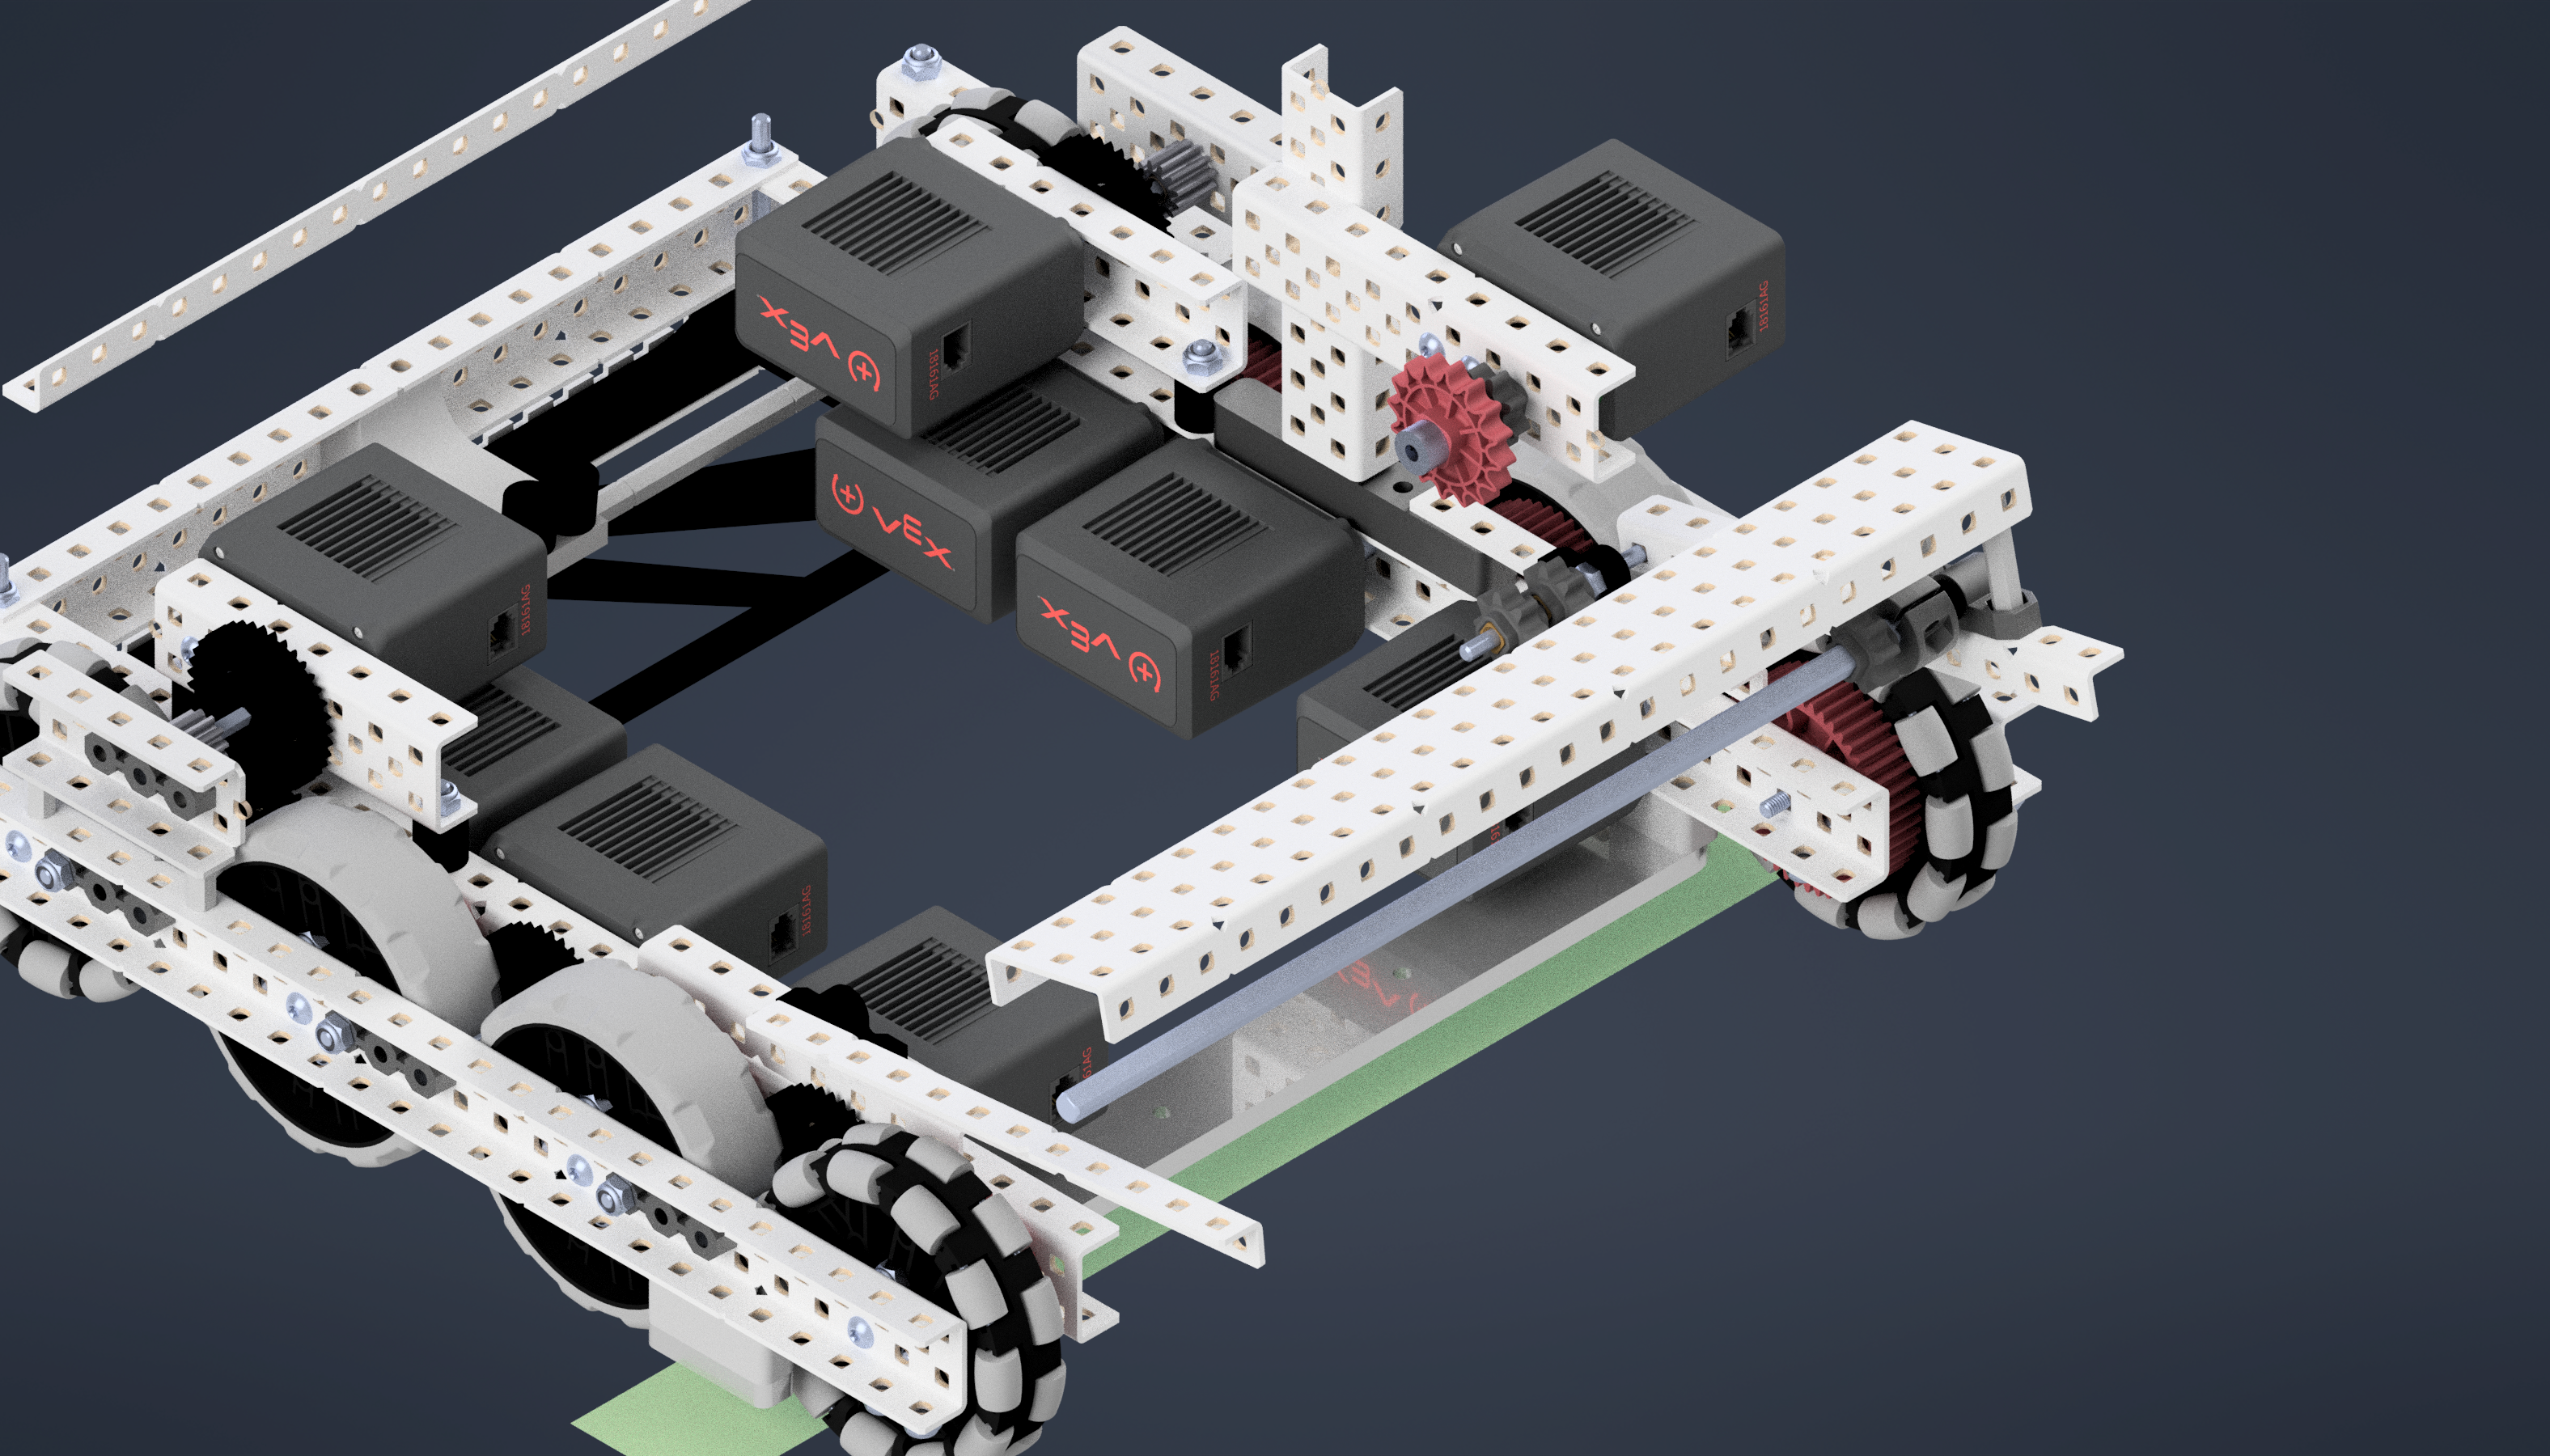
\includegraphics[width=\linewidth, height=5cm]{images/Intake/CAD_Intake.png} 
        \caption{CAD prototype} 
        \label{fig:CAD_Intake}
    \end{subfigure}
    % Main Caption for the whole figure
    \caption{Side-by-Side Comparison of Intake Architectures}
    \label{fig:comparison_view}
\end{figure}

With design considerations in mind, iteration 1 of the intake was developed with a chain driven motor with a direct 600 rpm. Note that the intake, when lowered, is outside of the required 15". While this would normally be a problem, allowing the intake to pivot lets us raise the intake to be within 15" when starting a match.
\newline

\subsection{Testing Design: Iteration 1}
A Ramp was designed and printed to have a curve that the blocks would be able to follow when acquired. Although initial testing went well, after further review, several key issues were found. 
\newline

\subsubsection{Problems}
These are the issues that were discovered after initial testing and review of iteration 1

\begin{itemize}
    \item The overall length of the intake was too long. When observing a potential starting position, the edge of the flexwheels was approximately .5" outside the required size constraint. 
    \item  If the flexwheels position was to be moved back in order to fit the size constraint, it would be right above the ramp leading to the intake being lifted to much.
\end{itemize}

\subsection{Design Solution}
Let us first address the most critical issue, the length. It is unavoidable that we must reduce the length of the intake as seen in \ref{fig:Intake_Shorten}. We moved the intake one hole or .5" back in order to be within the size constraint.

\begin{figure} [H]
    \centering
    \includegraphics[width=0.5\linewidth]{images/Intake/Intake_Shorten.jpg}
    \caption{Intake moved back one hole or .5"}
    \label{fig:Intake_Shorten}
\end{figure}

\begin{figure} [H]
    \centering
    \includegraphics[width=0.5\linewidth]{images/Intake/Intake_No_Ramp.jpg}
    \caption{Updated intake with no ramp}
    \label{fig:Intake_No_Ramp}
\end{figure}


\section{Conveyor System}
\textbf{Objective:} Establish the full \textit{conveyor} roller system (bottom intake stage and upper redirect stage) to begin prototyping and fine tuning the overall design.
\newline

\textbf{Problem Definition:} To transition from CAD theory to physical implementation, we must validate the conveyor’s interaction with the game elements in both stages. The primary challenge is tuning roller spacing and positioning of the rollers in order to balance secure control and compression for grabbing and redirection with enough clearance to prevent jams, stalls, or unintended ejection as the element transfers upward. Although many design choices will be shared between stages, the bottom and top geometries influence the game element differently, so both must be evaluated together to confirm consistent, reliable feeding through the entire conveyor path, and as such we will go through iterations for both the top and bottom stages to showcase the difference between both stages. However, when discussing the tests and problems for both stages, those sections will be combined to streamline solutions. 
\newline

    \subsubsection{Solution Requirements}
\begin{itemize}
    \item \textbf{Mechanism Constraint:} The mechanism must be able to conform to the shape of the block in order to increase the surface area of contact. 
    \item \textbf{Grip Constraint:} The material used must provide enough friction to ensure that blocks do not slide downward or away from the desired location.
    \item \textbf{Material Constraint (Rubber Band Sprockets):} The Rollers must utilize rubber band sprockets in order to easily fit the other constraints while still being prototyped.  
\end{itemize}


\subsection{Bottom Stage}
\subsubsection{Iteration 1}
    Following the engineering design process, we first began brainstorming on a whiteboard which can be seen in \ref{fig:Conveyor_Brainstorm}

    \begin{figure}
        \centering
        \includegraphics[width=0.5\linewidth, height = 10 cm]{images/White Board Drawings/Brainstorm of conveyor .jpg}
        \caption{Brainstorming of Conveyor}
        \label{fig:Conveyor_Brainstorm}
    \end{figure}

    Following our design choices from earlier, we decided to use rubber band rollers to determine the correct height needed for the rollers. A 5by C-Channel was held in an approximate location and an axle was used with an old custom sprocket from Over Under to determine compression. 
    

\begin{figure}[H]
    \centering
    % First Image (Left)
    \begin{subfigure}{0.3\textwidth} % Increased to 0.45 so images are larger
        \centering
        % height=6cm forces vertical size match
        \includegraphics[width=\linewidth, height=6cm]{images/Intake/First Roller.jpg} 
        \caption{Iteration one of Roller.}
        \label{fig:First_Roller}
    \end{subfigure}
    \hspace{2cm} % <--- REPLACES \hfill TO REDUCE GAP
    % Second Image (Right)
    \begin{subfigure}{0.3\textwidth} % Increased to 0.45
        \centering
        % height=6cm to match the left image
        \includegraphics[width=\linewidth, height=6cm]{images/Intake/First Roller Ball.jpg} 
        \caption{Roller with ball.} 
        \label{fig:First_Roller_Ball}
    \end{subfigure}
    
    % Main Caption for the whole figure
    \caption{First prototype of first roller.}
    \label{fig:First_Roller_Proto}
\end{figure}

    After finding the approximate location for the first roller, we approached the mounting system using tower cranes as an inspiration. By establishing a main tower, we can easily choose positions at various lengths and heights while prototyping. 

\begin{figure} [H]
    \centering
    \includegraphics[width=0.5\linewidth]{images/Intake/Tower Crane Method.jpg}
    \caption{First Instance of "Crane Method" being used}
    \label{fig:Crane_Method}
\end{figure}

    With the intake and first roller established we began to realize that although we can test compression and the intake. It would be impossible to fully test and break the conveyor system until the upper and bottom stages were made. Jamming, Friction, and Capacity could not be determined or tested without those two stages. 

    \begin{figure} [H]
        \centering
        \includegraphics[width=0.5\linewidth]{images/Intake/Second Roller.jpg}
        \caption{Second Roller attached}
        \label{fig:Second Roller}
    \end{figure}


\subsection{Top Stage}

\subsubsection{Iteration 1}
    Following the engineering design process, A very rudimentary layout for the top stage was added using 1by's and standoffs in order to establish a four bar lift as seen in \ref{fig:Top_Stage} the initial design was inspired by Tenton \cite{bib:tntn_reveal} Abs and anti-slip matting was used to build a rudimentary ramp to establish the next steps in the design process.
    
    \begin{figure} [H]
        \centering
        \includegraphics[width=0.35\linewidth, height = 9cm]{images/Intake/Top Stage.jpg}
        \caption{Added top stage and prototype ramp.}
        \label{fig:Top_Stage}
    \end{figure}

Two towers were also attached to the back of the chassis to continue our approach with the "Crane Method", allowing us to mount the stationery center roller for the curve as seen in \ref{fig:Top_Stage} and \ref{fig:Center_Ramp}

\begin{figure} [H]
    \centering
    \includegraphics[width=0.5\linewidth]{images/Intake/Hood and Center Roller.jpg}
    \caption{Center Roller and ramp attached}
    \label{fig:Center_Ramp}
\end{figure}

\subsection{Testing Design: Trail and Error}
    During testing following our initial selection of roller sizes, overall intake performance worked; However, serval issues were found. 
\newline

\subsubsection{Problems}
These are the issues that were discovered after initial testing and review of Iteration 1 leading to less than desired results and some key issues. 

\begin{itemize}
    \item While the rollers did work intaking the blocks when trying to score into the long goal, it was found that the last roller did not have enough compression in order to effectively score the blocks into the goal.
    \item  Compression was too much and as a result caused jamming of the conveyor before the bot could intake the maximum amount of blocks the bot could hold.
    \item The separation between the center roller and the upper stage leads to a gap in the rollers, leading to a tendency for blocks to be spit out prematurely. 
\end{itemize}

\subsubsection{Design Solutions}
    Addressing the first problem: We opted to increase the size of the roller for this iteration in order to confirm that our overall idea could work in the first place, and a previous designed sprocket was used in iteration 1 as seen in \ref{fig:Bigger_Top_Roller} allowing four blocks to be scored in the long goal. 

    \begin{figure} [H]
        \centering
        \includegraphics[width=0.7\linewidth]{images/Intake/New Top Roller.jpg}
        \caption{A bigger size sprocket was added to the top stage (yellow sprocket)}
        \label{fig:Bigger_Top_Roller}
    \end{figure}

    % ------------------ Long Goal Block Scoring vs Roller Diameter ------------------
\begingroup
\setlength{\tabcolsep}{4pt}      % tighter columns
\renewcommand{\arraystretch}{1.1}% a little more row height
\footnotesize

\begin{longtable}{@{}ccccc p{0.38\textwidth}@{}}
\caption{Long Goal Block Scoring vs Roller Diameter (1 block per attempt; success = fully in)}\label{tab:longgoal_rollerdiameter}\\
\toprule
Roller Dia. (in) & Attempts (n) & Scored (fully in) & Missed & Success (\%) & Notes \\
\midrule
\endfirsthead

\toprule
Roller Dia. (in) & Attempts (n) & Scored (fully in) & Missed & Success (\%) & Notes \\
\midrule
\endhead

1.50 & 30 & 20 & 10 & 66.7 & More slip; occasional partial insert \\
1.75 & 30 & 24 & 6  & 80.0 & More consistent engagement \\
2.25 & 30 & 27 & 3  & 90.0 & Best alignment + push-through behavior \\
\bottomrule
\end{longtable}
\endgroup

\subsubsection{Solution Brainstorm}

Furthermore, to address the dead-zones that were found in the system, the current design was revisioned as seen in \ref{fig:OG_Master_Sketch} in which a constant radius ramp was brainstormed that would lead to a constant path of compression on the ball allowing us to fine tune friction, with jamming and dead-zones all in one. For this design, we will use a 28\degree straight ramp that ends at the beginning of the ramp curve.
    \begin{figure}  [H]
        \centering
        \includegraphics[width=0.5\linewidth]{images/Intake/Iteration2.png}
        \caption{Geometry Proposal for Iteration 2}
        \label{fig:OG_Master_Sketch}
    \end{figure}


\subsection{Bottom Stage}

    \subsubsection{Iteration 2}
Following the initial sketch and brainstorm, a more realistic design sketch was curated in Inventor as seen in \ref{fig:Master_SKetch_V1}. With this sketch using the minimum and maximum radius of a block, we are able to realize the ideal size of rubber band wheels, the idealized curve of a ramp and the needed size for a pivot sprocket in order to reduce dead zones, friction, and the perfect amount of compression. 

    \begin{figure}  [H]
        \centering
        \includegraphics[width=0.5\linewidth]{images/Intake/CAD master sketch.png}
        \caption{Iteration 2 Bottom Stage Geometry Sketch}
        \label{fig:Master_SKetch_V1}
    \end{figure}


To assume the right position for the first roller, a custom print was made in order to reach the appropriate geometry as seen in \ref{fig:Roller_Custom}. With this print, we were able to attach bottom stage rollers in the right position when following the elevation of the ramp and blocks. By using the correct amount, we now have a standard position for the rollers and to Tune compression so that different size sprockets can be tested. 


\begin{figure} [H]
    \centering
    \includegraphics[width=0.7\linewidth, height= 7 cm]{images/Intake/Roller Custom Motor Cap.jpg}
    \caption{Custom Mount for roller and motor.}
    \label{fig:Roller_Custom}
\end{figure}


\subsection{Top Stage}

    \subsubsection{Iteration 2}
    The top stage will be drastically different than iteration 1. With this new design, we seek to solve a critical gap problem of iteration 1 through the use of flex wheels. One of the main problems with iteration 1 is that our upper stage would have a tendency to spit balls out accidentally when pivoted to the height required to score on the long goal. This is due to not pivoting about the largest sprocket on the robot. For context, the previous iteration would start with the upper stage sprockets parallel with the largest sprocket on the bottom stage. However, the upper stage frame did not pivot about the center of this sprocket. Instead, the upper stage pivoted on a tower that was positioned roughly 3" back. With this geometry, the gap between the final bottom stage sprocket and the first upper stage sprocket would grow as the angle increased. Thus, a \textit{deadzone} would appear between these two, which was not consistent nor ideal. It is worth noting however, that as this geometry allowed the robot to have increased reach that equated to the size of the gap. Additionally, we seek to make the upper stage a four bar that pivots about the largest sprocket in the system. This sprocket will be called the \textit{pivot sprocket}. The four bar linkage will be wider in the bottom to members to accommodate the gearbox that will continuously power all the sprockets together from the two motors on the bottom stage. The two upper members of the four bar linkage will be more narrow than the bottom two. By making the four bar narrower on the top, we want the the narrow section to effectively funnel the balls so that the upper stage is less prone to jamming. Moreover, making the upper stage a four bar will allow us to have an indexer mechanism that will remain perpendicular to the field tiles in any scoring position. This four bar however, will not have the compression hood mounted on the top linkage, but rather mounted on standoffs on the bottom linkage. In doing this, compression can remain the same regardless of the upper stage angle as seen in \ref{fig:V1_Top_Stage}.

\begin{figure} [H]
    \centering
    \includegraphics[width=0.5\linewidth]{images/Intake/v1 top stage.jpg}
    \caption{1st iteration of top stage}
    \label{fig:V1_Top_Stage}
\end{figure}

A Ziptie was added at the end of the four bar lift in order to test jamming and dead-zones when motion stopped in the system. 

\begin{figure} [H]
    \centering
    \includegraphics[width=0.5\linewidth]{images/Intake/ziptie door.jpg}
    \caption{prototype four bar lift}
    \label{fig:ZipTie_Door}
\end{figure}

A new ramp was added to replace the abs piece; this was done in order to start standardizing the testing of several sub-systems when working together. 

\begin{figure} [H]
    \centering
    \includegraphics[width=0.5\linewidth]{images/Intake/ramp v1.jpg}
    \caption{Ramp from the bottom}
    \label{fig:placeholder}
\end{figure}

\subsection{Testing Design: Iteration 2}
    Iteration 2 can be said to be the first step of a very long staircase to complete the project in terms of design, although it had issues in its design and implementation, it gave a standardization to our prototype, allowing for more accurate testing and tuning to happen. Let us review the issues we found and the solutions we are looking forward to.  
    \newline

    \subsubsection{Problems}
        These are the issues that were discovered after initial testing and review of iteration 2 leading to less than desired results and some key issues. 

        \begin{itemize}
            \item The balls jammed at the end of the top stage.
            \item The balls would get caught in the curve between the bottom stage and the top stage.
            \item  The intake did not apply enough force to push the ball into the goal if there are already balls inside the goal.
        \end{itemize}
    
    \subsubsection{Design Solutions}
    We are going to adjust the tension of the intake so that the balls can move more freely inside the intake. This will make it to where the balls will move at a greater speed, therefore having a greater momentum which should kill two birds with one stone.

    \subsubsection{Solution Brain Storm}
    Instead of fixed points, we could use TPU connection points that would allow more movement than a rigid material.

    \subsubsection{Iteration 3}
    While innovative, testing of Iteration 2 demonstrated that rubber band rollers are superior to small flex wheels for our intake mechanism. Consequently, we have decided to significantly revise the geometry. Analysis of the first two iterations indicates that the optimal sprocket positions lie within a 1" diameter of their current coordinates. We are confident that fine-tuning these sprocket locations within this tolerance will resolve the jamming issues while maintaining target performance. A rough drawing was created to illustrate the path that the team wants to proceed in and it can be seen in \ref{fig:Iteration2vs3}.
    
\begin{figure}
    \centering
    \includegraphics[width=0.5\linewidth]{images/Intake/Original Master Sketch.jpg}
    \caption{Iteration 2 geometry vs. Iteration 3 proposed geometry}
    \label{fig:Iteration2vs3}
\end{figure}
    
    
    A New ramp was made following the problems in iteration 2 in order to have a continuous curve for the pivoting top stage

\begin{figure}[H]
    \centering
    \begin{subfigure}[b]{0.48\linewidth}
        \centering
        \includegraphics[width=\linewidth]{images/Intake/Ramp V2.jpg}
        \caption{Mesh Bottom}
        \label{fig:ramp_v2}
    \end{subfigure}\hfill
    \begin{subfigure}[b]{0.48\linewidth}
        \centering
        \includegraphics[width=\linewidth]{images/Intake/Installed Ramp V2.jpg}
        \caption{Mesh Bottom Installed}
        \label{fig:installed_ramp_v2}
    \end{subfigure}
    \caption{Intake with mesh}
    \label{fig:ramp_pair}
\end{figure}

    \newpage
    New "oncloud" mech that was used in order to have compression when either the ball is at its minimum radius and maximum radius, allowing us to have consistent pressure on the main pivoting. 

  \begin{figure}[H]
    \centering
    \begin{subfigure}[b]{0.48\linewidth}
        \centering
        \includegraphics[width=\linewidth]{images/Intake/on-cloud v1.jpg}
        \caption{Caption}
        \label{fig:oncloud_v1}
    \end{subfigure}\hfill
    \begin{subfigure}[b]{0.48\linewidth}
        \centering
        \includegraphics[width=\linewidth]{images/Intake/on cloud mounts.jpg}
        \caption{Caption}
        \label{fig:oncloud_mounts}
    \end{subfigure}
    \caption{Caption}
    \label{fig:oncloud_pair}
\end{figure}

    
\subsection{Top Stage}

    \subsubsection{Iteration 3}

        Reworked stop stage without 3D printed arms, added 3D printed bearings, and redid rollers for compression along with a continuous curve ramp. This continuous ramp, slides along our "oncloud", akin to shingles. This allows for compression to be the same along the curve of the bot regardless if the upper stage is up or down.
        
\begin{figure}[H]
    \centering
    \begin{subfigure}[b]{0.48\linewidth}
        \centering
        \includegraphics[height=8cm,keepaspectratio]{images/Intake/Top stage Iteration 3.jpg}
        \caption{Caption}
        \label{fig:top_stage_iter3}
    \end{subfigure}\hfill
    \begin{subfigure}[b]{0.48\linewidth}
        \centering
        \includegraphics[height=8cm,keepaspectratio]{images/Intake/Top stage iteration 3 pivoting.jpg}
        \caption{Caption}
        \label{fig:top_stage_iter3_pivot}
    \end{subfigure}
    \caption{Caption}
    \label{fig:top_stage_iter3_pair}
\end{figure}

    
\subsection{Testing Design: Iteration 3}
    Iteration 2 is the first step of a very long staircase, completing the project in terms of design. Although it had issues in the design and implementation, it gave a standardization to our prototype, allowing for more accurate testing and tuning to occur. Let us review the issues we found and solutions we are looking forward to.  
    \newline

    \subsubsection{Problems}
        These are the issues that were discovered after initial testing and review of iteration 3 leading to less than desired results and some key issues. 

        \begin{itemize} 
            \item  Blocks had a tendency to offset causing blocks to be side by side leading to multiple issues
            \item  The original design for the pivot utilized two screw joints on each side of the pivot using a brass insert to rotate. However, this inevitably caused to PLA sprocket's center to get reamed out as seen in 
        \end{itemize}
\begin{figure}[htbp]
    \centering
    \begin{minipage}{0.45\textwidth}
        \centering
        \includegraphics[width=\linewidth]{images/Intake/Reamed Out Sprocket.jpg}
        \caption{Damaged \textit{pivot sprocket} with brass instert}
        \label{fig:ReamedSprocket}
    \end{minipage}\hfill
    \begin{minipage}{0.45\textwidth}
        \centering
        \includegraphics[width=\linewidth]{images/Intake/Reamed Out Sprocket 2.jpg}
        \caption{Reamed \textit{Pivot sprocket}}
        \label{fig:ReamedSprocket2}
    \end{minipage}
\end{figure}
    \subsubsection{Design Solutions}
        We plan to optimize the intake curvature to increase capacity by one to two additional balls. Additionally, we will integrate a sorting "door" mechanism. This system will allow us to eject opposing alliance colors and provide a pass-through option to score on the high goal from either a front or back approach.

        To prevent balls from offsetting during transfer, we proposed adding a polycarbonate guide to the top stage pivot. However, the current pivot design—relying on a standard VEX screw joint through the sprocket—is problematic. The bending moment applied by the upper stage creates excessive friction on the sprocket, inhibiting rotation. We must design a solution that isolates the structural pivot force from the rotating sprocket to ensure smooth operation.
    \subsubsection{Solution Brain Storm}
        Building on our success with custom wheels, we intend to fabricate a custom aluminum axle for the central pivot, adapting the design shown in \ref{fig:traction_axle}. By lathing an axle that is tapped on both ends, we can mount it as a rigid structural member—effectively treating it as a reinforced standoff. Crucially, this configuration decouples the pivot loads from the sprocket rotation (provided the sprockets ride on independent bearings). This isolation is essential, as we anticipate the upper stage will endure significant stress, particularly during descoring maneuvers.
    \subsubsection{Iteration 4}
        Iteration 4 will retain the sprocket geometry established in Iteration 3 because testing confirmed its efficacy. The primary failures of the previous iteration were attributed to the pivot joint instability, the absence of a color sorter, and ball jamming. We hypothesize that the jamming issues stem from the static compression surfaces, such as the ABS curve, rather than the sprocket layout. Consequently, we will focus on tuning these static geometries and investigating alternative materials to reduce friction along the ball path.
        
\subsection{Top Stage}

    With the upper stage starting to reach its final prototype it was decided that a polycarbonate piece would be used to align the blocks from the pivot to the upper stage in order to form a more coherent flow through the bot. 

    \subsubsection{Iteration 4}

        \begin{figure}[H]
    \centering
    \begin{subfigure}[b]{0.4\linewidth}
        \centering
        \includegraphics[width=\linewidth]{images/Intake/poly carb aligner.jpg}
        \caption{Added new polycarbonate piece for guiding blocks}
        \label{fig:Polycarb_guide}
    \end{subfigure}
    \hfill
    \begin{subfigure}[b]{0.4\linewidth}
        \centering
        \includegraphics[width=\linewidth]{images/Intake/Poly carb aligner tilted.jpg}
        \caption{Tilted upper stage to express block guiding}
        \label{fig:Polycarb_guide_tilted}
    \end{subfigure}
    \caption{Polycarbonate guide concept for block alignment}
    \label{fig:Polycarb_guide_pair}
\end{figure}


\section{Pivot}


\section{Wing}







\newpage
\chapter{Senior Design Integration and Analysis}

While the Prototype Evolution chapter established the robot's architecture, this chapter details the specific critical design choices revisions, tuning, and refinement to establish a superior rating across all categories. 
\newline

\section{Drivetrain Iteration 1: Legacy Revision}
\textbf{Objective:} Establish a 10 motor drive train based on a 8 motor prototype chassis envisioned from previous seasons.
\newline

\textbf{Problem Definition:} 
Designing and machining a custom 10-motor drivetrain from scratch requires significant lead time (CAD, CNC machining, Assembly). However, by simultaneously prototyping with a previous year chassis, we are able to effectively have a split development. Where once a final iteration is made on the prototype, a almost perfect design can be made for the Senior version. 
\newline

\subsection{Drivetrain Components}
    One of the first issues that the team addressed was how do we fit 5 motors in a space that was taken up by 4 motors. As you can see in \ref{fig:motor_cap_and_prototype} we opted to create a custom 3D print to attach all 5 motors. In this print, we also designed it so that all motors can be hot-swapped for any issues that are discovered during use. 

    \begin{figure}[H]
    \centering
    \begin{subfigure}[b]{0.48\linewidth}
        \centering
        \includegraphics[width=\linewidth]{images/drivetrains/Right Drive Side motor cap .png}
        \caption{Custom Motor Cap and Attachment}
        \label{fig:custom_motor_cap}
    \end{subfigure}
    \hfill
    \begin{subfigure}[b]{0.48\linewidth}
        \centering
        \includegraphics[width=\linewidth]{images/drivetrains/Prototype Half view .png}
        \caption{Prototype attachment}
        \label{fig:prototype_attachment}
    \end{subfigure}
    \caption{Motor cap design and prototype attachment overview}
    \label{fig:motor_cap_and_prototype}
\end{figure}

    When we compare both mounting styles side by side, as shown in \ref{fig:Real Estate view}, the five motor footprint is nearly the same as the space the prototype required. This means we can move forward with re-envisioning a chassis that supports a full ten motor drivetrain without introducing major packaging conflicts. By treating the prototype chassis as a proven baseline, we preserve the geometry and constraints that already worked while expanding capacity. Just as importantly, the prototype testing clarified critical details like motor clearance, fastener access, and serviceability that can now be designed from the start.

    \begin{figure} [H]
        \centering
        \includegraphics[width=0.5\linewidth]{images/drivetrains/Real estate view .png}
        \caption{Comparing Taken Space between each style}
        \label{fig:Real Estate view}
    \end{figure}

    \subsubsection{Traction Wheels}

        A criteria that has been imposed on the senior design is that it shall be designed in order to be able to manufacture most parts. This includes the wheels that both bots will be using. This section will go over decisions that were made in order to develop said wheels; from type of rubber to use to which components should be reused/bought rather than manufactured ourselves. 
        \newline

        \begin{table}[H]
        \centering
        \caption{Traction wheel tread material selection (cast elastomers)}
        \label{tab:tread_selection}

        \begingroup
        \small
        \setlength{\tabcolsep}{6pt}
        \renewcommand{\arraystretch}{1.15}

        \begin{tabularx}{\textwidth}{@{}c p{0.34\textwidth} c Y c@{}}
        \toprule
        Option & Material & Shore A & Rationale & Status \\
        \midrule
        A & \textbf{BBDINO clear silicone mold rubber} (1:1 by volume) & \textbf{30A} &
        Chosen for simple, repeatable casting and high compliance for traction. Clear material helps verify mixing and spot bubbles during pours. &
        \textbf{Chosen} \\

        B & Polyurethane (cast urethane) & 60A--70A &
        Common tread material with solid grip and improved wear life compared to very soft silicone. &
        Alternative \\

        C & Polyurethane (cast urethane) & 80A--90A &
        Higher durability and stable diameter under load, typically less peak grip than softer treads. &
        Alternative \\

        D & TPU-style elastomer (cast/molded) & 70A--95A &
        Very tough and abrasion resistant, but traction varies strongly with formulation and hardness. &
        Alternative \\
        \bottomrule
        \end{tabularx}

        \endgroup
        \end{table}

        

    As you can see in \ref{tab:tread_selection} a silicone rubber was selected with a shore hardness of 30A, this was chosen because of the high compliance the materials have allowing for more surface area between the field and the wheel, and with it being used last year for flexwheels, we have prior experience with durability and functionality making it a easy choice for this component. 

 \begin{figure}[H]
    \centering
    \begin{minipage}[t]{0.48\linewidth}
        \centering
        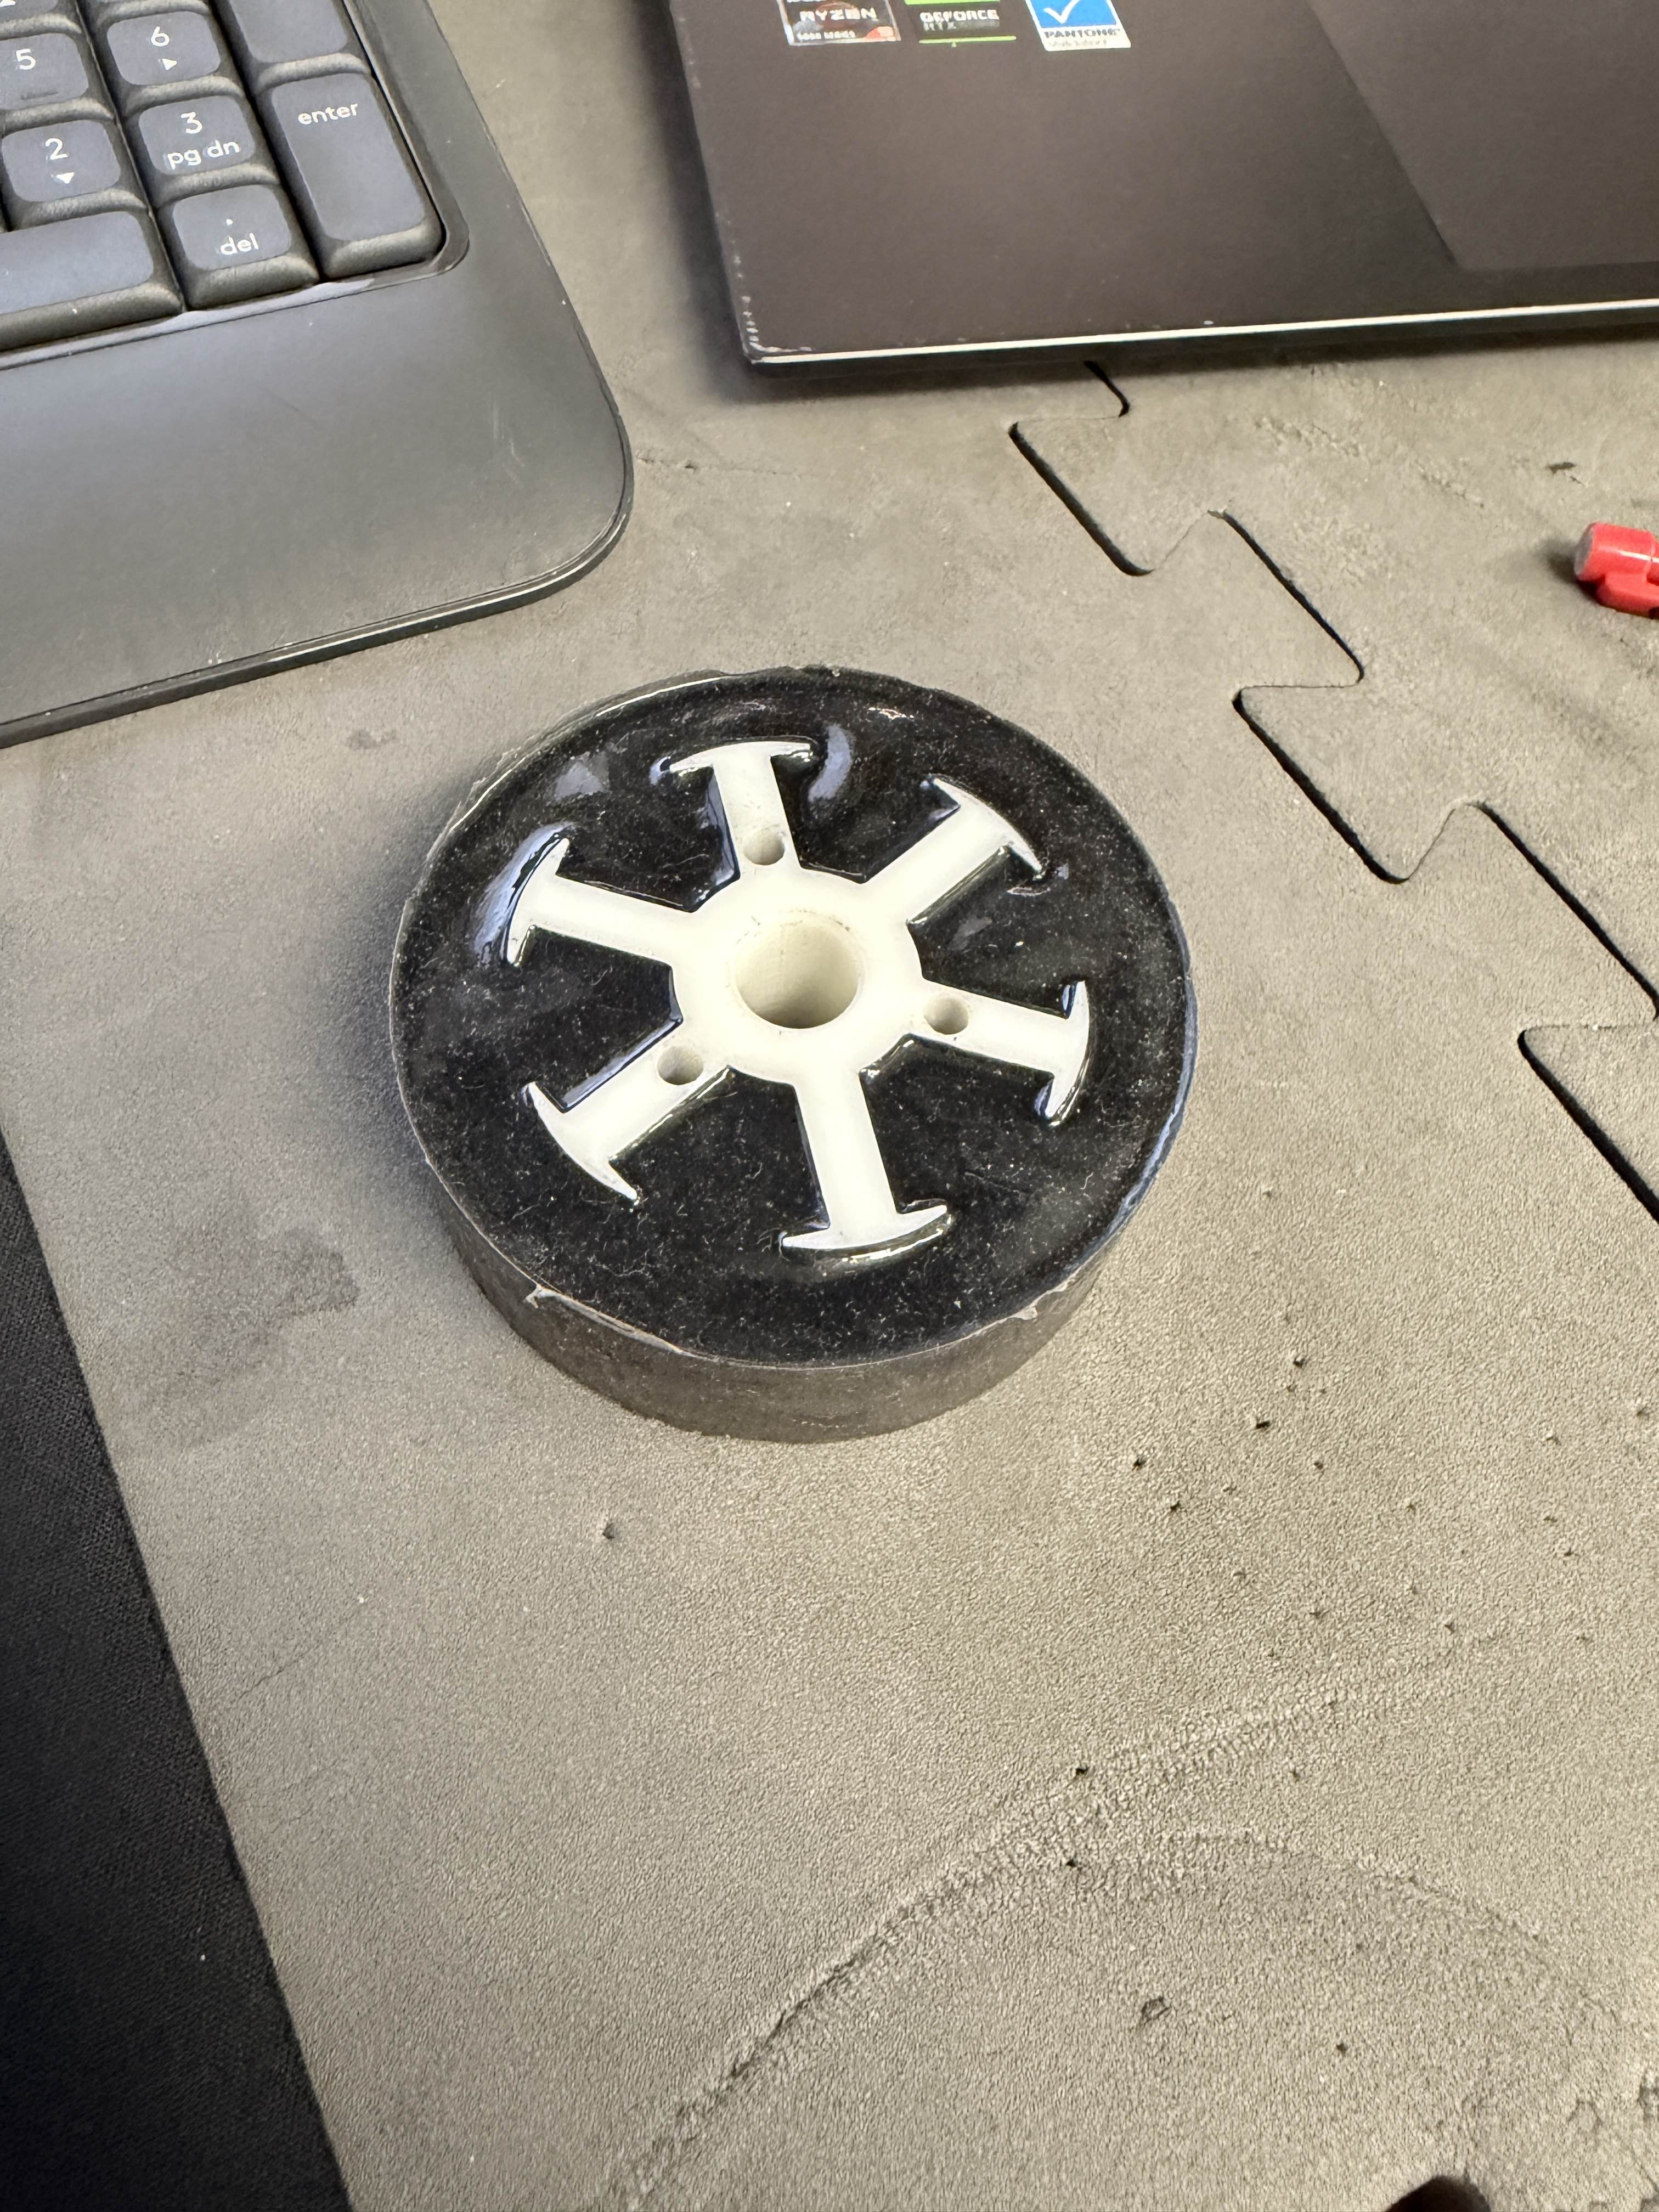
\includegraphics[width=\linewidth,height=0.25\textheight,keepaspectratio]{images/drivetrains/First iteration traction wheel.jpg}
        \caption{First iteration of traction wheel}
        \label{fig:first_iteration_traction_wheel}
    \end{minipage}\hfill
    \begin{minipage}[t]{0.48\linewidth}
        \centering
        \includegraphics[width=\linewidth,height=0.25\textheight,keepaspectratio]{images/drivetrains/expanded view traction wheel.jpg}
        \caption{Expanded view of traction wheel}
        \label{fig:expanded_traction_wheel}
    \end{minipage}
\end{figure}

    During the first iteration of the traction wheels a spoke design commonly found in real life wheels was designed and was casted on top of which can be found in \ref{fig:first_iteration_traction_wheel} and \ref{fig:expanded_traction_wheel}, which show both the 3D printed spokes and the casted silicone. Although it lead to a working design the overall weight was much greater then a VEX traction wheel. This lead to iteration 2 of the traction wheel which can be seen in \ref{fig:traction_wheel_hub_views}
    
   \begin{figure}[H]
    \centering
    \begin{subfigure}[b]{0.48\linewidth}
        \centering
        \includegraphics[height=5cm,keepaspectratio]{images/drivetrains/Traction Wheel Hub.png}
        \caption{Front of traction wheel hub}
        \label{fig:traction_wheel_hub_front}
    \end{subfigure}
    \hfill
    \begin{subfigure}[b]{0.48\linewidth}
        \centering
        \includegraphics[height=5cm,keepaspectratio]{images/drivetrains/Back of Traction Wheel Hub.png}
        \caption{Gear side of traction wheel hub}
        \label{fig:traction_wheel_hub_back}
    \end{subfigure}
    \caption{Traction wheel hub views}
    \label{fig:traction_wheel_hub_views}
\end{figure}

    A Hub was created in order to attach the casted component to the drivetrain and give it a rigid spine to have a functional wheel which can be seen in \ref{fig:traction_wheel_hub_views}. In the figure you can also see that the gear is a part of the hub, allowing us to save space during the construction of the drivetrain along with giving us room to play with how big and small the driven and drive gears can be and still achieve 450 rpm. Creating a custom wheel to allowed us to directly integrate bearings into the wheel to reduce friction from the system.  

\begin{figure}[H]
    \centering
    \includegraphics[height=0.35\textheight,keepaspectratio]{images/drivetrains/traction wheel mold.jpg}
    \caption{Mold of the traction wheel}
    \label{fig:traction_mold}
\end{figure}

    Following the casting of the wheel it was assembled in a 4 part process. The Overall Hub is split into 3 parts a Outer plate, A center Hub and the gear plate. While the actual casted part is added on with the gear plate at the same time. 
    
    \begin{figure} [H]
        \centering
        \includegraphics[width=0.5\linewidth]{images/drivetrains/Assembled Traction Wheel.jpg}
        \caption{Fully assembled traction wheel}
        \label{fig:Assembled Traction Wheel}
    \end{figure}


    In \ref{fig:traction_mold} the 3D printed mold that was designed to directly fit on to the hub, ensuring proper alignment, consistent tread thickness, and repeatable manufacturing. Using a 3D printed mold allows us to use rapid iteration, maintaining a tight tolerance between the hub and the cast, which reduces the likelihood of slippage or delamination when in use.

\begin{table}[H]
\centering
\caption{Measured sliding (kinetic) traction coefficient from pull testing}
\label{tab:traction_mu_k}
\begin{tabular}{lccc}
\hline
\textbf{Test} & \textbf{Pull Force, $F$ (lb)} & \textbf{Normal Load, $W$ (lb)} & \textbf{Sliding Coefficient, $\mu_k = F/W$} \\
\hline
Test A & 14.53 & 20.66 & 0.70 \\
Test B & 18.50 & 16.125 & 1.15 \\
\hline
\end{tabular}
\end{table}

\noindent
\textbf{Traction Testing and Calculation:}
Wheel traction was evaluated using a pull test. A known normal load was applied to the driven wheel(s), and the pulling force was measured while the wheel was \emph{already slipping} (continuous sliding/spinning). Because the measurement was taken during sliding, the reported values correspond to the kinetic (sliding) coefficient of friction, $\mu_k$.

\begin{equation}
\mu_k = \frac{F_f}{N}
\label{eq:muk_def}
\end{equation}

\noindent
In this setup, the measured pull force is the friction force ($F_f = F$) and the normal force is the applied load on the driven wheel(s) ($N = W$). Using consistent pound-force units, Eq.~\eqref{eq:muk_def} reduces to:

\begin{equation}
\mu_k = \frac{F}{W}
\label{eq:muk_pulltest}
\end{equation}

\noindent
For Test A,
\begin{equation}
\mu_k = \frac{14.53}{20.66} = 0.703 \approx 0.70
\end{equation}
and for Test B the load was converted from $16~\text{lb}~2~\text{oz}$ to pounds:
\begin{equation}
W = 16 + \frac{2}{16} = 16.125~\text{lb}
\end{equation}
which gives
\begin{equation}
\mu_k = \frac{18.50}{16.125} = 1.147 \approx 1.15
\end{equation}

Following our testing and calculations we have a increase of 64\% in the coefficient of friction. This is a significant increase compared to the value of last years bot, meaning that we are significantly harder to push around or be bullied compared to other bots we may see. 
\newline

\subsubsection{Omni Wheels}

   The design for the Omni wheels was a more straightforward path, since there were only a few downsides to the standard VEX omni wheels:
\begin{itemize}
    \item The wheel was a bit heavy, so a total of four wheels added noticeable weight.
    \item The wheel was also somewhat bulky when designing last year's omni pods. In order to make them direct-driven, gears had to be affixed to the wheels, which increased the overall packaging size and complexity. 
\end{itemize}

\begin{figure}[H]
    \centering
    \includegraphics[width=0.5\linewidth,height=0.5\textheight,keepaspectratio]{images/drivetrains/Assemled omni hub.jpg}
    \caption{Assembled Omni Wheel Hub}
    \label{fig:Assembled Omni Hub}
\end{figure}

    By 3D printing these hubs it reduced the overall weight along with the complexity of the pods allowing for a smaller packaging size as seen in \ref{fig:Assembled Omni Hub}. It was also decided that we would reuse rollers from vex omni wheels due to legality of using outside assemblies. It also allowed for bearings to be directly used in the wheel leading to a reduced friction load increasing overall speed and torque. 

   \begin{figure}[H]
    \centering
    \begin{minipage}[t]{0.48\linewidth}
        \centering
        \includegraphics[width=\linewidth,height=0.25\textheight,keepaspectratio]{images/drivetrains/IMG_0103.jpg}
        \caption*{(a) View 1}
    \end{minipage}\hfill
    \begin{minipage}[t]{0.48\linewidth}
        \centering
        \includegraphics[width=\linewidth,height=0.25\textheight,keepaspectratio]{images/drivetrains/IMG_0104.jpg}
        \caption*{(b) View 2}
    \end{minipage}

    \caption{Assembled omni pod (two views)}
    \label{fig:assembled_omni_pod}
\end{figure}

    Much like the traction wheel the omni pods were made in 4 parts; a outer shell, inner hub, gear plate, and omni rollers. You can see a fully assembled pod in \ref{fig:assembled_omni_pod}. while there isn't much testing that we can do for the pod other than the reduction of weight which came to around a 15\% reduction in overall weight and around a 20\% reduction in overall size. 
    \newline


    \subsubsection{Braking System}

    Compared to last year, our traction wheels provide much more traction. In order to maximize this, we are adding a brake system that is similar to a design we used last year. Doing this allows us to hold any position on the field without being easily moved.
    \newline

    Following last year's system, we used a piston to mate to a driven gear which then locks the drivetrain and does not allow any m,ovement in the wheels.

 \begin{figure}[H]
    \centering
    \begin{subfigure}[t]{0.48\linewidth}
        \centering
        \includegraphics[width=\linewidth,height=0.25\textheight,keepaspectratio]{images/Senior Design/Gear Grabber.png}
        \caption{Component to mesh into gears}
        \label{fig:gear_grabber}
    \end{subfigure}\hfill
    \begin{subfigure}[t]{0.48\linewidth}
        \centering
        \includegraphics[width=\linewidth,height=0.25\textheight,keepaspectratio]{images/Senior Design/Brake Attachment.png}
        \caption{Fixture component for brake system}
        \label{fig:brake_attachment}
    \end{subfigure}

    \caption{Gear grabber and brake attachment components}
    \label{fig:gear_grabber_brake_attachment}
\end{figure}

    Redesigning last years brake system, we arrive at \ref{fig:gear_grabber_brake_attachment}. \ref{fig:gear_grabber} is a component that we use to catch the teeth of the gears in order to remove any motion in the gear. Although \ref{fig:brake_attachment} is the point of attachment to the sliding gear mesh and the piston to the chassis without interference with other systems. 
    \newline


    
    \subsection{Full Integration}

    This section will go over integrating each separate part together into a functional subsystem of the robot and the individual parts needed to fully integrate starting with the driven system. While the driven gears are attached to the individual wheels because of their custom pitch diameter and teeth, it was required that we create custom gears for the motors in order to achieve our desired 450 rpm. 

    \begin{figure} [H]
        \centering
        \includegraphics[width=0.5\linewidth, height= .25\textheight, keepaspectratio]{images/drivetrains/18T gear.png}
        \caption{The drove gear of the system}
        \label{fig:18T gear}
    \end{figure}

    By using custom gears, we were able to operate in a much tighter space allowing for a more modular and compact design. With the compact design, we were able to bring each of the components closer, leading to only a quarter inch gap between each wheel, as seen in \ref{fig:spaced drivetrain}. 

    \begin{figure} [H]
        \centering
        \includegraphics[width=0.5\linewidth]{images/Senior Design/Spaced Drivetrain.png}
        \caption{Spaced wheels and gears}
        \label{fig:spaced drivetrain}
    \end{figure}

    By designing a fully custom drivetrain, it allows us to take the liberties that where previously unavailable to us. For example, we were able to design around having each driven axle have bearings, which allows a reduced friction and machining custom axles that perfectly allow the wheels to spin and be in the right position without the use of spacers, which allows a cleaner and more modular design all of which can be seen in \ref{fig:spaced drivetrain}

    \begin{figure}[H]
    \centering
    \begin{subfigure}[t]{0.48\linewidth}
        \centering
        \includegraphics[width=\linewidth,height=0.25\textheight,keepaspectratio]{images/Senior Design/Drive Axle Traction.png}
        \caption{Machined axle for traction wheels}
        \label{fig:traction_axle}
    \end{subfigure}\hfill
    \begin{subfigure}[t]{0.48\linewidth}
        \centering
        \includegraphics[width=\linewidth,height=0.25\textheight,keepaspectratio]{images/Senior Design/Drivetrain axle bearings.png}
        \caption{Off-the-shelf bearings used on the outer drive plates}
        \label{fig:drive_bearings}
    \end{subfigure}

    \caption{Traction axle and drivetrain bearing components}
    \label{fig:traction_axle_and_bearings}
\end{figure}

    With the use of bearings and custom machined axles found in \ref{fig:traction_axle} and \ref{fig:drive_bearings}. we were able to reduce friction to a large amount, leading to more power being applied to the drive train rather than the use of energy being used to overcome friction. This will lead to a quicker acceleration and a shorter time to reach max velocity.  

   \begin{figure}[H]
    \centering
    \begin{subfigure}[t]{0.48\linewidth}
        \centering
        \includegraphics[width=\linewidth,height=0.25\textheight,keepaspectratio]{images/Senior Design/Outer Plate.png}
        \caption{Outer plate of drivetrain}
        \label{fig:outer_plate}
    \end{subfigure}\hfill
    \begin{subfigure}[t]{0.48\linewidth} 
        \centering
        \includegraphics[width=\linewidth,height=0.25\textheight,keepaspectratio]{images/Senior Design/Pocketed Inner plate.png}
        \caption{Geometry translation from prototype}
        \label{fig:inner_plate}
    \end{subfigure}\
    \caption{Drivetrain plate components}
    \label{fig:drivetrain_plates}
\end{figure}

    By having a prototype bot with working geometry, it becomes incredibly easy to design and manufacture working parts. This can be seen in \ref{fig:inner_plate}. Since every known bolt, axle, and any other fixture location is known, we can prototype advanced designs and still be accurate. The outer plate or \ref{fig:outer_plate} holds bearings and the axle attachment points.

    \begin{figure} [H]
        \centering
        \includegraphics[width=0.7\linewidth]{images/Senior Design/Assembled Drive Half.png}
        \caption{Fully assembled drive halve}
        \label{fig:Drivetrain Half}
    \end{figure}

    \ref{fig:Drivetrain Half} shows a fully assembled half of the drivetrain with placement/fixture point for every bolt and axle needed from the prototype bot that transitioned to the senior design. This allows for very limited problems when designing and building as can already be seen in comparison in the amount of problems found in the prototype chapter vs the senior design chapter. 
    \newline

    \subsubsection{Bracing Components}

        This section covers components made for the drivetrain in order to enhance the structure of it, along with bringing the design into a functional state. 


            \paragraph{Back Brace}\mbox{}\\

            
           \textbf{Overview:} Working from last year, the team knew that a component was needed in order to fully make our drivetrain rigid and square. However, with a fully custom bot it provides unique challenges on how do we integrate a custom piece with no known attachment points? This was solved in our prototype design by utilizing the prototype bot we eliminate that problem.
            \newline
            
           \textbf{Design:} when designing the drivetrain a initial cap was made in the back in order to box each side of the drive as seen in \ref{fig:Originial Chassis Block}. Although it did box each side it did nothing to limit the row in the drivetrain and did not provide a way to attach each half together.
            \newline

        \begin{figure} [H]
            \centering
            \includegraphics[width=0.5\linewidth]{images/Senior Design/oringial Chassis block.png}
            \caption{Initial cap used for the drivetrain}
            \label{fig:Originial Chassis Block}
        \end{figure}

        \textbf{Design Iteration 2:} After the initial design a bar was added between each half as seen in \ref{fig:Chassic Block Stretch Method}. This attached each half together allowing for a functional drivetrain as a whole. However it still allowed more play then desired by a team and following placement of components on the prototype a few designs needed to be added in order to meet the same geometry and sizing. 
        \newline

        
        \begin{figure} [H]
            \centering
            \includegraphics[width=0.5\linewidth]{images/Senior Design/Rear chassis block stretch method .png}
            \caption{Added brace in between each block}
            \label{fig:Chassic Block Stretch Method}
        \end{figure}


        \textbf{Design Iteration 3:}  Following a finalized design on the prototype each component was added to back brace in order to simplify construction and manufacturing. For example, in \ref{fig:V1 rear chassis block} we added mounting positions for the ramp along with a attachment point for the intake ramp. Bracing was also added in order to provide support to the span of the brace in order to reduce bowing along with a point added in the center to attach our odometry system. 
        

        \begin{figure} [H]
            \centering
            \includegraphics[width=0.5\linewidth]{images/Senior Design/Final rear chassis block.png}
            \caption{V1 of the finalized rear chassis block}
            \label{fig:V1 rear chassis block}
        \end{figure}

        \textbf{Design Iteration 4:} In the final iteration of the rear chassis block we took inspiration from a car. For example a car rear bumper is made to crumble in order to reduce stress. However, following the logic of a truck where the rear bumper is backed by the frame. This logic can be seen in \ref{fig:V2 rear Chassis Block} where we subtracted the thickness of the rear chassis block and added a metal bumper made of aluminum in order to absorb impacts and provide a rigid backbone to the whole print as seen in \ref{fig:Aluminium backbone}.

\begin{figure}[H]
    \centering
    \begin{subfigure}[b]{0.48\linewidth}
        \centering
        \includegraphics[width=\linewidth,height=0.22\textheight,keepaspectratio]{images/Senior Design/Final Final Rear Chassis Block.png}
        \caption{V2 of final rear chassis Block}
        \label{fig:V2 rear Chassis Block}
    \end{subfigure}
    \hfill
    \begin{subfigure}[b]{0.48\linewidth}
        \centering
        \includegraphics[width=\linewidth,height=0.22\textheight,keepaspectratio]{images/Senior Design/Full back brace assembly.jpg}
        \caption{Assembled back brace with aluminum backbone}
        \label{fig:Aluminium backbone}
    \end{subfigure}
    \caption{Rear chassis block and back brace assembly}
    \label{fig:rear_block_and_backbrace}
\end{figure}

        \paragraph{Chassis Block and Cross Bar}\mbox{}\\

        Taking another note from last year, although having a back brace helps reduce sway and play adding another brace closer to the front almost eliminates it entirely. However, the same as the back brace developing a method to attach the brace is the majority of the problem. 
        \newline

        \textbf{Chassis block Iteration 1:} When first designing the chassis block with how limited space was in between each will it would be hard to design around it. Heatset inserts were used in order to attach it to both the inner and outer drive plates while the outcropping on top of the main block as seen in \ref{fig:rear_block_and_backbrace} was used in order to align the whole setup using the outer part of the drive bearings located on the out plate as seen in \ref{fig:Drivetrain Half}
        
        \begin{figure}
            \centering
            \includegraphics[width=0.5\linewidth]{images/Senior Design/Chassis Block.png}
            \caption{3D Printed insert between wheels in order to attach a cross bar}
            \label{fig:Chassis Block}
        \end{figure}

        as seen in\ref{fig:Attached Chassis Block} the block squeezes in between each wheel well and perfectly aligns both sides of the drive and provides a attachment points for a crossbar. 

        \begin{figure} [H]
            \centering
            \includegraphics[width=0.5\linewidth]{images/Senior Design/Attached Chassis Block.png}
            \caption{Constrained chassis block}
            \label{fig:Attached Chassis Block}
        \end{figure}

    \textbf{Cross Bar Iteration 1:} The design for the initial cross bar was simplistic in nature it was made in order to attach both sides and have a functional drivetrain up in running without compromising on integrity and overall rigidity. This cross bar can be seen in \ref{fig:V1 Cross Bar} where the holes on either end where made in order to attach the cross bar to the chassis block via heat-set inserts.

    \begin{figure} [H]
        \centering
        \includegraphics[width=0.5\linewidth]{images/Senior Design/Cross bar v1.jpg}
        \caption{V1 of the senior design cross bar}
        \label{fig:V1 Cross Bar}
    \end{figure}

        \textbf{Cross Bar Iteration 2:} The innovations made to Iteration 2 were mostly on accident. For example iteration two added a chamfer to the bottom edge of the cross bar, this was added due to how perfectly in level the bar was with the parking zone. So a chamfer was added in order to help the bot lift in order to park. While counter sunk bolts where added in order to fully make the bottom of the bot flush and eliminate the parking barrier being caught on bolts. all of these features can be seen in \ref{fig:V2 Cross Bar}. 

    \begin{figure}[H]
        \centering
        \includegraphics[width=0.5\linewidth]{images/Senior Design/Cross bar v2.jpg}
        \caption{V2 of the senior design cross bar}
        \label{fig:V2 Cross Bar}
    \end{figure}

        \textbf{Cross Bar Iteration 3:} The only iterations added to version 3 were holes added to the center in order to attach a ramp to the bot these changes can be seen in \ref{fig:V3 Cross Bar}.

    \begin{figure}[H]
        \centering
        \includegraphics[width=0.5\linewidth]{images/Senior Design/Cross bar v3.jpg}
        \caption{V3 of the senior design cross bar}
        \label{fig:V3 Cross Bar}
    \end{figure}

     \textbf{Cross Bar Iteration 4:} This iteration 4 is currently the final iteration for the cross bar. It brought in closer the ramp attachment points along with added four points in order to attach a railing mount in for our match loading mechanism. 

    \begin{figure} [H]
        \centering
        \includegraphics[width=0.75\linewidth]{images/Senior Design/Final Cross Bar.png}
        \caption{Final iteration of cross bar}
        \label{fig:Final Cross Bar}
    \end{figure}


\section{Lower Stage}

    This section will cover translating the lower stage from the prototype to the senior design, and the designs and components used in order to achieve the same geometry
    \newline
    
    \subsection{Brainstorming}

        One of the main issues we ran into while developing the senior design was: How do we attach different prints and other components to each other? We addressed this issue with brass heatset inserts as the main attachment point along with the press fitting. In \ref{fig:Heat Insert Block} We tested the tolerance and found that a perfect size hole would be .217" diameter hole. 

    \begin{figure} [H]
        \centering
        \includegraphics[width=0.5\linewidth]{images/Senior Design/Heat insert block.jpg}
        \caption{Heatset Insert Block used to test tolerance}
        \label{fig:Heat Insert Block}
    \end{figure}

    We then tested the durability of the heat inserts, a concern was raised that while heat inserts were versatile, would they provide enough strength when in a print to hold together under load. This was done by inserting a screw into heatset inserts and then applying a load to the test block as seen in \ref{fig:Heatset Block Weighted}.

    \begin{figure} [H]
        \centering
        \includegraphics[width=0.5\linewidth]{images/Senior Design/Heatset insert weighted.jpg}
        \caption{Tested Heatset Insert Block being weighted}
        \label{fig:Heatset Block Weighted}
    \end{figure}

    Upon testing the strength of the heatset inserts, we found that we were limited by the bucket holding all the weight since it failed before the heatset insert block could even begin to bulge, providing sufficient reason to utilize this throughout our entire design.
    \newline

    \subsection{Motor Attachment}

        The prototype already confirmed the correct geometry for the lower stage motor attachment, so the Senior Design work is mainly a clean translation of that layout into the final CAD and manufacturing-ready parts. We reused the existing motor cap designs and kept the same axle positions to preserve the proven alignment and performance. At the same time, the Senior Design version is laid out to give us more flexibility in how components are mounted, leaving extra room to adjust brackets, spacing, and fastener locations without changing the core geometry.

    \begin{figure} [H]
        \centering
        \includegraphics[width=0.5\linewidth]{images/Senior Design/Lower Stage with bearing.jpg}
        \caption{Lower Stage Motor Attachment with Bearings}
        \label{fig:Lower Stage Bearings}
    \end{figure} 

    \ref{fig:Lower Stage Bearings} shows the lower stage prototype motor/axle attachment, with the main 3D-printed mount using an integrated bearing and a separate motor cap piece. Since the prototype already confirms the correct axle positions and alignment, the Senior Design work is mainly rebuilding this same geometry cleanly in the final CAD. We are reusing the motor cap design and keeping the axle centerlines locked in, while adjusting the surrounding mounting features to give more room and flexibility for how everything is fastened and positioned in the final assembly.

   \begin{figure}[H]
    \centering
    \includegraphics[height=0.45\textheight, keepaspectratio]{images/Senior Design/Lower Stage no bearing.jpg}
    \caption{Lower Stage Motor Attachment With No Bearings}
    \label{fig:Lower Stage No Bearings}
\end{figure}

    \ref{fig:Lower Stage No Bearings} shows the updated lower stage motor/axle attachment after revising the prototype. We removed the integrated bearing because it was causing fitment issues with standard axles and instead shifted to a setup that better matches our normal shaft hardware and tolerances. In this version, we also added a previously missed mounting point for attaching a piston, giving us a clean, rigid location to integrate the actuator without changing the core geometry of the lower stage.


    \begin{figure} [H]
        \centering
        \includegraphics[width=0.8\linewidth]{images/Senior Design/Lower Stage Motor Attachment.png}
        \caption{Lower Stage With motor attachment}
        \label{fig:Lower Stage Motor Attachment}
    \end{figure}

    Rather than using heatset inserts to mount the component to the aluminum inner plate, we opted to press fit parts of the 3D printed component into the pocketed areas of the plate as seen in \ref{fig:Lower Stage Bearings}. The final attachment can be seen in \ref{fig:Lower Stage Motor Attachment} Where the component is pressed in and then screws are attached to secure it fully. 


    \begin{figure} [H]
        \centering
        \includegraphics[width=0.5\linewidth]{images/Senior Design/Right Side no bearings.png}
        \caption{Right side geometry component}
        \label{fig:Right side Geometery}
    \end{figure}

        The same geometry was from \ref{fig:Lower Stage No Bearings} and mirrored it with minor changes as the fundamental geometry is the same allowing for a quicker implementation on the bot the final design can be seen in \ref{fig:Right side Geometery}. 

        \begin{figure} [H]
            \centering
            \includegraphics[width=0.5\linewidth]{images/Senior Design/Lower stage full assembly .png}
            \caption{Cadded assembly of the bottom stage components}
            \label{fig:Bottom stage assembly}
        \end{figure}

        The full design was constrained and tolerance as seen in \ref{fig:Bottom stage assembly} this allowed us to create custom spacers that would reduce the overall weight on the bot and for a quicker assembly when building. This also allowed us to plan how to run chain and sprockets in order to fully drive the lower stage fully. 

\section{Odometry}
    
To accurately track our robots' movement across the field during the autonomous and driver control periods, we had to come up with an improved method of odometry. In previous seasons, our team has used the same wheel encoders with success but had trouble with the overall placement and design of the wheel module. Problems with our last season's odometer pods were that they were too bulky in size, lacked stroke length, and were too difficult to integrate into an existing chassis. We knew that we wanted to create a completely modular design that's easy to install on any configuration. To eliminate these issues, our team had to switch to a more custom and universal mechanism that could allow our tracking to work nearly perfectly.
\newline

    When brainstorming for this new iteration we came up with the most important issues that the new design would address:
\begin{itemize}
    \item Reduce the footprint that pods take up on the underside of the chassis
    \item Increase design durability without sacrificing size constraints
    \item Allow for more diverse mounting locations
    \item Decrease unnecessary slop with wheel and encoder rotations
    \item Increase the stroke length so that the odometers will always make contact with the ground even while the chassis is elevated
\end{itemize}

These improvements would allow the robots to accurately track their position relative to the field and game elements even when an unexpected event occurs such as being lifted up by another bot or game element. From our experience, it is best to design every subassembly to perform under any conditions so the drivers don't have to worry about mechanical failure. With past odometer assemblies being fragile, we knew durability would be a characteristic to focus on.
\newline

\subsubsection{1. Problem Statement}

Standard omnidirectional wheels (including Mecanum and standard Omni-wheels) often suffer from "discontinuous contact" with the ground due to the gaps between passive rollers. This discontinuity creates vertical and horizontal vibrations during operation, which can degrade sensor accuracy (particularly odometry and IMU readings) and reduce traction consistency.
\newline

\textbf{Objective:} Design a custom wheel that maintains continuous ground contact to minimize vibration and increase the surmountable bump height, improving the robot's stability and climbing ability.
\newline

\subsubsection{2. Research \& Technical Justification}

Our design is grounded in the research paper \textit{"Design of Continuous Alternate Wheels for an Omnidirectional Mobile Robot"} by Kim et al. (2003).

\begin{itemize}
    \item \textbf{The Concept:} The paper proposes a "Continuous Alternate Wheel" (CAW) where large and small rollers are arranged alternately around the hub. Unlike standard designs where rollers are spaced apart, the CAW ensures that as one roller leaves the ground, the next one (of a different radius/position) is already making contact.
\newline
    \item \textbf{Design Math:} The paper establishes that the geometry of the wheel relies on the number of rollers and the intersection of their profiles. While the paper explores designs with n=4 and n=6, we have adapted this theory to a 5-roller configuration to balance roller size with the complexity of the printed assembly.
\newline
    \item \textbf{Gap Minimization:} The primary goal of this geometry is to eliminate the gap between rollers. As stated in the research, "this feature of no gap... is important in reduction of vibration during the wheel operation".
\end{itemize}
\newline

\subsubsection{3. Design Specification \& Implementation}

We translated the theoretical CAW model into a manufacturable design using 3D printing and laser-cut manufacturing techniques available to our VexU team.

\paragraph{A. Component Architecture}

\begin{itemize}
    \item \textbf{Hub \& Spokes (PLA):}
    \begin{itemize}
        \item We designed 5 custom PLA spokes that serve as the central skeleton of the wheel.
        \item \textit{Function 1:} These spokes act as the retainer for the "inner" rollers (standard omni-wheel rollers).
        \item \textit{Function 2:} The outer ends of each spoke are geometrically shaped to project the inner race geometry for the bearings. This allows the spoke itself to act as the stationary axle for the outer TPU rollers.
    \end{itemize}
    \item \textbf{Outer Rollers (TPU):}
    \begin{itemize}
        \item \textbf{Material:} Printed in TPU (Thermoplastic Polyurethane) to provide high friction and impact dampening.
        \item \textbf{Innovation:} These rollers feature print-in-place bearings. Instead of pressing in commercial bearings, the bearing geometry is printed directly inside the TPU roller during fabrication. This reduces part count and allows for custom bearing sizing that perfectly matches the PLA spoke projection.
        \item \textbf{Geometry:} The outer roller profile follows the "barrel" shape required to match the wheel circumference, ensuring the transition from inner to outer roller is smooth.
    \end{itemize}
    \item Containment Plates (Stainless Steel)\textbf{:}
    \begin{itemize}
        \item Two 16-gauge stainless steel plates sandwich the entire assembly.
        \item These plates handle the structural load, preventing the PLA spokes from flexing under the robot's weight. This addresses the concern raised in the research that "a urethane roller is not solid enough to prevent deformation" without proper support.
    \end{itemize}
\end{itemize}

\paragraph{B. Fastening}

The assembly is compressed and secured using M2 bolts, passing through the steel plates and PLA spokes. This creates a rigid "composite" structure where the steel takes the tension/compression and the printed parts handle the complex geometry.
\newline

\subsubsection{4. Prototype \& Construction}

The following images detail the construction process of the CAW module.
\newline

\begin{figure}[H]
    \centering
    \includegraphics[width=0.5\linewidth]{images/Senior Design/TPU Bearing roller.jpg}
    \caption{Bearing and Roller Integration}
    \label{fig:placeholder}
\end{figure}


\textit{A close-up of the custom TPU outer roller. The print-in-place bearing is visible in the center. The use of TPU allows the roller to deform slightly over obstacles, improving traction, while the internal geometry remains rigid enough to rotate freely on the PLA spoke.}
\newline

\begin{figure}[H]
    \centering
    \includegraphics[width=0.5\linewidth]{images/Senior Design/CAW Final.jpg}
    \caption{Full Assembly}
    \label{fig:placeholder}
\end{figure}


\textit{The fully assembled Continuous Alternate Wheel. You can see the alternating pattern of the 5 larger TPU rollers (black, outer) and the 5 smaller rollers (grey, inner) retained by the PLA spokes. The stainless steel plates visible in the center hub bind the spokes together, ensuring the wheel can withstand the torque requirements of competitive play.}
\newline

\subsubsection{5. Expected Performance \& Future Testing}

Based on the FEM (Finite Element Method) analysis in the source text, we expect the stress distribution to be highest at the supporter of the outer roller. Our use of 16-gauge steel plates specifically addresses this by reinforcing the hub area.
\newline

\textbf{Testing Plan:}

\begin{enumerate}
    \item \textbf{Vibration Test:} Drive the robot on hard tiles and measure accelerometer noise compared to standard omni-wheels.
    \item \textbf{Bump Test:} Verify the wheel's ability to cross Vex field barriers (e.g., tape lines, small obstacles) without significant heading deviation, testing the "surmountable bump" theory.
    \item \textbf{Durability:} Stress test the print-in-place bearings under load to ensure the TPU/PLA interface does not degrade over time.
\end{enumerate}
\newline

\subsubsection{6. Conclusion}

This design successfully implements the Continuous Alternate Wheel theory  into a VexU-legal form factor. By utilizing hybrid manufacturing (3D printing + laser cutting), we have created a wheel that theoretically offers superior smoothness and traction compared to off-the-shelf components.























\chapter{Daily Logs}

\section{8/21/25}
    Team discussed what they wanted their custom omni wheels to look like, and they started designing a rough draft of the wheels weighing the pros and cons of the designs.
\newline

\begin{figure} [H]
    \centering
    \includegraphics[width=0.5\linewidth]{images/drivetrains/custom omni wheel.png}
    \caption{This is the first iteration of a custom omni wheel.}
    \label{fig:placeholder}
\end{figure}


 \section{8/23/25}
    Kavin, Gavin, and McKenzie were assigned to create a test bed to help transition members from high school to University level Vex Robotics, along with giving a platform for incoming programmers to develop on. 
\newline

\section{9/3/25}
    Cooper printed the first prototype of their custom omni wheel and assembled it. 
\newline

    Collin started on the CAW \cite{bib:design_CAW} first tolerance testing the casing to hold the omni roller.
\newline

\begin{figure}[H]
    \centering
    \includegraphics[width=0.5\linewidth]{images/drivetrains/omni roller disassembled.jpg}
    \caption{This is the individual pieces used for the omni rollers.}
    \label{fig:placeholder}
\end{figure}

\begin{figure}[H]
    \centering
    \includegraphics[width=0.5\linewidth]{images/drivetrains/odom omni roller.jpg}
    \caption{This is the first omni roller Collin made to test the tolerances.}
    \label{fig:placeholder}
\end{figure}

\section{9/5/25}
    Juan and Ryan assembled the drivetrain components and ensured proper gear alignment, while Cooper verified smooth power transmission between stages. The printed gears were tested under load to check for any premature wear, while adjustments were made to mounting points to reduce unnecessary stress on the gear teeth. Minor spacing changes were implemented to improve meshing between the gears, while maintaining the compact profile of the drivetrain assembly. Further testing was conducted to confirm consistent rotation without binding, while observing any deformation that could occur during extended use.
\newline

\begin{figure}[H]
    \centering
    \includegraphics[width=0.5\linewidth]{images/drivetrains/omni wheel gears.jpg}
    \caption{These are the first iteration of the gears made which will go on the wheels.}
    \label{fig:placeholder}
\end{figure}

\section{9/7/25}
    Juan continued refining the chassis layout, ensuring proper spacing for drivetrain components and future subsystem mounting. Cooper finalized the omni wheel print settings to improve durability and dimensional accuracy. Hunter inspected the traction wheel after curing, verifying proper bonding between the hub and outer tread. Minor adjustments were made to the mold design to improve consistency in future traction wheel casts. The assembled wheel was then mounted and tested to confirm proper fitment within the drivetrain system.

\begin{figure}[H]
    \centering
    \includegraphics[width=0.5\linewidth]{images/drivetrains/final omni wheel design.jpg}
    \caption{This is the finished omni wheel design.}
    \label{fig:placeholder}
\end{figure}

\begin{figure}[H]
    \centering
    \includegraphics[width=0.5\linewidth]{images/drivetrains/traction wheel mold.jpg}
    \caption{This is the Traction Wheel rubber mold Cooper designed.}
    \label{fig:placeholder}
\end{figure}

\begin{figure}[H]
    \centering
    \includegraphics[width=0.5\linewidth]{images/drivetrains/traction wheel assembled.jpg}
    \caption{This is the fully assembled Traction wheel alongside the motor cap that Juan designed.}
    \label{fig:placeholder}
\end{figure}

\section{9/8/25}
    Juan verified proper fitment of the motor group cap to ensure secure mounting to the chassis. Cooper assisted in assembling the motor group to confirm alignment between the cap and drivetrain components. Minor adjustments were made to the design to improve clearance for wiring and fasteners. The printed caps were then installed and inspected for any interference during rotation. Additional testing was conducted to ensure the cap maintained rigidity under load.
\newline

\begin{figure}[H]
    \centering
    % First Image (Left)
    \begin{subfigure}{0.4\textwidth}
        \centering
        % Added height=5cm to force vertical size match
        \includegraphics[width=\linewidth, height=5cm]{images/drivetrains/5 motor cap front.jpg} 
        \caption{Front view of the 5 motor cap hub.}
        \label{fig:placeholder}
    \end{subfigure}
\hspace{2cm} % <--- REPLACES \hfill TO REDUCE GAP    % Second Image (Right)
    \begin{subfigure}{0.4\textwidth}
        \centering
        % Added height=5cm to match the left image
        \includegraphics[width=\linewidth, height=5cm]{images/drivetrains/5 motor cap back.jpg} 
        \caption{Back view of the 5 motor cap hub.} 
        \label{fig:placeholder}
    \end{subfigure}
    % Main Caption for the whole figure
    \caption{Front and Back of 5 Motor Cap Hub}
    \label{fig:comparison_view}
\end{figure}

\section{9/14/25}
    Kavin and Gavin continued refining the sprocket geometry to improve retention of the rubber bands for the prototype robot. Cooper verified axle tolerances after lathing to ensure proper bearing fitment for the Senior Design drivetrain. Hunter assisted in inspecting the lathed axles to confirm alignment within the drivetrain assembly. Minor adjustments were made to the sprocket design to reduce unnecessary material while maintaining structural integrity. Both components were then reviewed separately prior to installation into their respective systems.
\begin{figure}[H]
    \centering
    % First Image (Left)
    \begin{subfigure}{0.3\textwidth}
        \centering
        % Added height=5cm to force vertical size match
        \includegraphics[width=\linewidth, height=5cm]{images/Intake/custom sprockets big.jpg} 
        \caption{4in Custom Sprockets}
        \label{fig:placeholder}
    \end{subfigure}
\hspace{2cm} % <--- REPLACES \hfill TO REDUCE GAP    % Second Image (Right)
    \begin{subfigure}{0.3\textwidth}
        \centering
        % Added height=5cm to match the left image
        \includegraphics[width=\linewidth, height=5cm]{images/Intake/custom sprockets.jpg} 
        \caption{2in Custom Sprocket} 
        \label{fig:placeholder}
    \end{subfigure}
    % Main Caption for the whole figure
    \caption{Custom Sprocket Rollers}
    \label{fig:comparison_view}
\end{figure}

\section{9/19/25}
    The assembled drivetrain side was inspected to ensure proper gear meshing and wheel alignment. Cooper assisted in verifying that the drivetrain components were securely mounted to prevent any unwanted movement during operation. Minor adjustments were made to spacing between components to improve overall fitment. Kavin and Gavin continued refining the angled brace design to ensure proper support for the intake structure. Additional test fitting was performed to confirm compatibility between the intake braces and chassis mounting points.
\newline
\begin{figure}[H]
    \centering
    \includegraphics[width=0.5\linewidth]{images/drivetrains/Assembled DT side.jpg}
    \caption{Assembled Drive Train side.}
    \label{fig:placeholder}
\end{figure}

\section{9/23/25}
    The installed braces were inspected to ensure proper alignment with the intake frame. Kavin assisted in verifying that all mounting points were securely fastened to prevent flex during operation. Minor adjustments were made to improve the fitment between the braces and surrounding structure. Additional test fitting was performed to confirm stability of the intake assembly. The intake structure was then reviewed to ensure compatibility with existing drivetrain components.. 
\newline
\begin{figure}[H]
    \centering
    \includegraphics[width=0.5\linewidth]{images/drivetrains/Prtotype bot angled braces.jpg}
    \caption{Progress of the prototype bot after adding the angled braces.}
    \label{fig:placeholder}
\end{figure}
\section{9/25/25}
    The assembled CAW was inspected to ensure proper alignment and structural rigidity. Juan continued refining the cross brace design to improve clearance for the traction wheels. Minor adjustments were made to the cutout geometry to prevent interference during rotation. Ryan assisted in reviewing the CAD model to confirm compatibility with existing drivetrain components. Additional test fitting was performed to verify proper integration of the cross brace within the custom drivetrain assembly.
\newline
\begin{figure}[H]
    \centering
    \includegraphics[width=0.5\linewidth]{images/drivetrains/Custom DT cutouts and braces.png}
    \caption{CAD model of the custom drive train with the cross brace and cutouts.}
    \label{fig:placeholder}
\end{figure}
\section{9/30/25}
    The completed prototype was inspected to ensure all subsystems were properly mounted and functioning as intended. Cooper verified that recent chassis modifications did not interfere with drivetrain components. Juan continued refining mounting points to improve overall structural support. Minor adjustments were made to the prototype to improve stability during operation. Additional testing was conducted to confirm compatibility between the prototype systems and the updated Senior Design chassis.
\newline
\begin{figure}[H]
    \centering
    \includegraphics[width=0.3\linewidth, height = 6cm]{images/drivetrains/Prototype bot.jpg}
    \caption{Completed first prototype bot}
    \label{fig:placeholder}
\end{figure}
%big gap in this we could talk about the addition of heat serts and the coutersunk bolts

\section{10/29/25}
    The printed components were inspected to ensure dimensional accuracy and proper fitment within the drivetrain assembly. Cooper assisted in verifying alignment between the drive plates and surrounding structural members. Minor adjustments were made to improve clearance for internal components. Juan continued assembling the drivetrain side to ensure structural integrity. Additional test fitting was performed to confirm compatibility with the funneling mechanism.
\newline
\begin{figure}[H]
    \centering
    \includegraphics[width=0.5\linewidth]{images/drivetrains/printed cutouts DT.jpg}
    \caption{Funneling system with new version of the drive plates.}
    \label{fig:placeholder}
\end{figure}

\section{10/30/25}
    The early intake components were assembled to evaluate roller placement and spacing. Cooper assisted in verifying proper alignment between the intake structure and drivetrain frame. Minor adjustments were made to improve the positioning of the first stage roller. Additional test fitting was performed to ensure smooth interaction with game objects. The intake assembly was then reviewed to confirm compatibility with the existing prototype configuration.
\newline
\begin{figure}[H]
    \centering
    \includegraphics[width=0.5\linewidth]{images/Intake/First Roller Ball.jpg}
    \caption{First roller of early iteration of intake}
    \label{fig:first roller}
\end{figure}

\section{11/5/25}
    The installed funnels were inspected to ensure proper alignment with the drivetrain assembly. Cooper verified that the funneling system did not interfere with wheel rotation or internal components. Minor adjustments were made to improve the positioning of the funnels within the chassis. Ryan and Juan continued refining the back brace design to improve overall structural support. Additional test fitting was performed to confirm compatibility between the back brace and existing drivetrain components.
\newline
\begin{figure}[H]
    \centering
    \includegraphics[width=0.45\linewidth]{images/drivetrains/Assembled custom DT side.jpg}
    \caption{Assembled custom Drive Train side with the new funneling system.}
    \label{fig:placeholder}
\end{figure}

\section{11/8/25}
    The assembled intake stage was inspected to ensure proper roller alignment and spacing. Juan verified that the intake structure was securely mounted to the chassis. Ryan assisted in reviewing the positioning of the intake components to prevent interference with surrounding frame members. Minor adjustments were made by Kavin to improve overall clearance between intake stages. Additional test fitting was performed by the group to confirm smooth interaction with game objects.
\newline
\begin{figure}[H]
    \centering
    \includegraphics[width=0.45\linewidth, height = 9cm]{images/Intake/Top Stage.jpg}
    \caption{First iteration of the top stage of the intake.}
    \label{fig:placeholder}
\end{figure}

\section{11/10/25}
    The installed back brace was inspected to ensure proper alignment with the drivetrain assembly. The team verified that the brace provided adequate structural support without interfering with internal components. Minor adjustments were made to improve fitment between the brace and surrounding frame members. Additional test fitting was performed to confirm stability during operation. The assembled drivetrain was then reviewed to ensure compatibility with future subsystem mounting.
\newline

\begin{figure}[H]
    \centering
    \includegraphics[width=0.5\linewidth]{images/drivetrains/Assembled Custom DT.jpg}
    \caption{First assembled custom Drive Train.}
    \label{fig:placeholder}
\end{figure}

\section{11/18/25}
    The installed motor caps were inspected to ensure proper alignment with the intake structure. Ryan verified that the caps provided adequate support for the first stage rollers. Juan assisted in reviewing the positioning to prevent interference with surrounding components. Cooper continued evaluating spacing between the secondary intake stages to improve overall fitment. Additional test fitting was performed by the group to confirm compatibility with the existing prototype configuration.
\newline

\begin{figure}[H]
    \centering
    \includegraphics[width=0.5\linewidth]{images/Intake/First stage intake with motor caps.jpg}
    \caption{First stage of the intake with the custom motor caps.}
    \label{fig:placeholder}
\end{figure}

\section{12/1/25}
    The printed pockets were inspected to ensure dimensional accuracy prior to installation. Juan evaluated the different sizes to determine optimal compression for intake performance. Minor adjustments were made to improve compatibility between the roller system and surrounding structure. Additional test fitting was performed to confirm proper alignment within the intake assembly. The various pocket sizes were then reviewed to identify the most effective configuration for consistent object intake.
\newline

\begin{figure}[H]
    \centering
    \includegraphics[width=0.5\linewidth]{images/Intake/Different size sprockets.jpg}
    \caption{Different size sprockets for rapid prototyping.}
    \label{fig:placeholder}
\end{figure}

\section{12/3/25}
The new screw joint mount was inspected to ensure proper alignment with the four-bar linkage. Juan verified that the updated joint reduced friction during operation compared to the previous axle-based setup. Minor adjustments were made to improve fitment within the intake assembly. Additional test fitting was performed to confirm smooth articulation of the second stage. The joint configuration was then reviewed to ensure compatibility with the existing intake structure.
\begin{figure}[H]
    \centering
    \includegraphics[width=0.35\linewidth,height=7cm]{images/Intake/Intake Pivot.jpg}
    \caption{Caption}
    \label{fig:placeholder}
\end{figure}
\newpage
\section{12/5/25}
    The mesh-wrapped rollers were inspected to evaluate grip consistency during operation. Juan verified that the mesh improved interaction between the rollers and game objects. Ryan and Kavin reviewed potential mounting configurations for the dynamic scoop. Cooper assisted in evaluating clearance between the scoop concept and existing drivetrain components. Additional discussion was conducted by the group to determine the most effective integration method for the rear scoop system. 
\newline

\begin{figure}[H]
    \centering
    \includegraphics[width=0.5\linewidth]{images/Intake/Mesh Rollers intake.jpg}
    \caption{Testing with mesh wrapped rollers for better and more consistent grip.}
    \label{fig:placeholder}
\end{figure}

\section{12/10/25}
    The hood prototypes were inspected to evaluate ball retention during loading. Juan and Ryan reviewed the different hood styles to improve consistency when fully loaded. Cooper verified that the match loading mechanism did not interfere with surrounding intake components. Hunter assisted in evaluating potential mounting configurations for the loading system. Additional test fitting was performed by the group to confirm compatibility between the hood and match loading mechanism.

\begin{figure}[H]
    \centering
    \includegraphics[width=0.5\linewidth]{images/Intake/New hood method.jpg}
    \caption{Final design of the intake hood.}
    \label{fig:placeholder}
\end{figure}

\section{12/14/25}
    The redesigned upper stage was inspected to ensure proper alignment with the intake assembly. Juan verified that the custom cross body axle provided adequate support during pivoting motion. Ryan assisted in evaluating the transition between the lower and upper intake stages. Minor adjustments were made to improve overall fitment within the intake structure. Additional test fitting was performed to confirm smooth articulation across the pivot point.
\newline

\begin{figure}[H]
    \centering
    \includegraphics[width=0.5\linewidth]{images/Intake/Updated upper stage.jpg}
    \caption{Redesigned upper stage pivot}
    \label{fig:placeholder}
\end{figure}

\section{12/16/25} 
    The lathed cross body axle was inspected to ensure proper dimensional accuracy. Cooper and Hunter verified that the axle fit securely within the intake pivot assembly. Juan evaluated the manufactured bottom crossbar to ensure compatibility with the chassis structure. Collin reviewed the updated inner drive plate design for proper alignment with drivetrain components. Additional test fitting was performed by the group to confirm integration between the newly fabricated parts. 
\newline
% 1. dual image cooper and hunter working on the lathe
\begin{figure}[H]
    \centering
    % First Image (Left)
    \begin{subfigure}{0.4\textwidth}
        \centering
        % Added height=5cm to force vertical size match
        \includegraphics[width=\linewidth, height=8cm]{images/Members/Cooper lathe.jpg} 
        \caption{Cooper lathing the cross body axle}
        \label{fig:placeholder}
    \end{subfigure}
    \hfill 
    % Second Image (Right)
    \begin{subfigure}{0.4\textwidth}
        \centering
        % Added height=5cm to match the left image
        \includegraphics[width=\linewidth, height=8cm]{images/Members/Hunter Lathe.jpg} 
        \caption{Hunter lathing the cross body axle} 
        %this looks like shart tbh you need to fix this
        %
        %
        %
        %
        %
        %
        %that photo looks like shart man its all distorted
        \label{fig:placeholder}
    \end{subfigure}
    % Main Caption for the whole figure
    \caption{Lathing the cross body axle}
    \label{fig:comparison_view}
\end{figure}
% 2. cross bar on the cnc 
\begin{figure}[H]
    \centering
    \includegraphics[width=0.5\linewidth]{images/drivetrains/CNC Cross bar.jpg}
    \caption{Bottom cross bar brace made from aluminum stock}
    \label{fig:placeholder}
\end{figure}
% 3. drive plate inner
\begin{figure}[H]
    \centering
    \includegraphics[width=0.5\linewidth]{images/drivetrains/Drive plate.jpg}
    \caption{New version of the inner drive plate.}
    \label{fig:placeholder}
\end{figure}

\section{1/8/26}
    The redesigned back cross brace was inspected to ensure proper alignment with the senior design chassis. Collin verified that the updated brace provided adequate structural support. Cooper evaluated the placement of the flex wheels to improve intake performance. Minor adjustments were made to ensure proper spacing between the flex wheels. Additional test fitting was performed by both to confirm compatibility with the intake assembly.
\newline
%back brace
\begin{figure}[H]
    \centering
    \includegraphics[width=0.5\linewidth]{images/drivetrains/Back brace.jpg}
    \caption{New version of the back brace for the senior design chassis}
    \label{fig:placeholder}
\end{figure}
%front photo with flex wheels
\begin{figure}[H]
    \centering
    \includegraphics[width=0.5\linewidth]{images/Intake/front flex wheels.jpg}
    \caption{First stage flex wheels on the senior design chassis}
    \label{fig:placeholder}
\end{figure}
\section{1/12/26}
    The initial descore mechanism was inspected to ensure proper range of motion. Juan verified that the geometry allowed for adequate extension during operation. Ryan assisted in evaluating the positioning of the mechanism relative to the intake assembly. Minor adjustments were made to improve overall fitment within the chassis. Additional testing was performed by both to confirm smooth articulation throughout the mechanism’s movement.
\begin{figure}[H]
    \centering
    % First Image (Left)
    \begin{subfigure}{0.4\textwidth}
        \centering
        % Added height=5cm to force vertical size match
        \includegraphics[width=\linewidth, height=8cm]{images/Other Mechs/Descore Arm Out.jpg} 
        \caption{Descore mech out}
        \label{fig:placeholder}
    \end{subfigure}
    \hfill 
    % Second Image (Right)
    \begin{subfigure}{0.4\textwidth}
        \centering
        % Added height=5cm to match the left image
        \includegraphics[width=\linewidth, height=8cm]{images/Other Mechs/Descore Mech Down.jpg} 
        \caption{Descore mech down} 
        \label{fig:placeholder}
    \end{subfigure}
    % Main Caption for the whole figure
    \caption{Descore Arm}
    \label{fig:comparison_view}
\end{figure}

\newpage
\section{1/15/26}
    The printed motor mount was inspected to ensure proper fitment with the intake assembly. Collin verified that the mount provided adequate support for the first row of flex wheels. Minor adjustments were made to improve alignment with surrounding components. Additional test fitting was performed to confirm compatibility within the intake structure. The motor mount was then reviewed to ensure stability during operation.
    \begin{figure}[H]
    \centering
    \includegraphics[width=0.5\linewidth]{images/Intake/Motor Mount for intake.jpg}
    \caption{Motor mount for the first row of flex wheels}
    \label{fig:placeholder}
\end{figure}

\newpage
\section{1/18/26}
    Ryan and Gavin adjusted the geometry of the descore arm to improve overall performance. Multiple arm angles were tested to evaluate functionality and determine the most effective configuration. These adjustments allowed for better positioning of the mechanism during operation. Testing focused on identifying an angle that provided consistent engagement while maintaining structural stability. The updated geometry was reviewed for integration with the existing intake system.
    \begin{figure}[H]
        \centering
        \includegraphics[width=0.35\linewidth,height=6cm]{images/Other Mechs/Descore mech new geometry.jpg}
        \caption{New geometry of the descore arm}
        \label{fig:placeholder}
    \end{figure}

\section{1/21/26}
    Ryan integrated a hook onto the descore arm to allow for functional testing of this iteration. This addition enabled the team to evaluate the mechanism’s ability to effectively engage with game elements during operation. Testing was conducted to assess overall performance and reliability of the updated design. Observations from these trials were used to inform future refinements of the descore mechanism.
    \begin{figure}[H]
        \centering
        \includegraphics[width=0.35\linewidth, height=6cm]{images/Other Mechs/Descore Hook.png}
        \caption{Descore arm hook}
        \label{fig:placeholder}
    \end{figure}

\newpage
\section{1/22/26}
    Juan began prototyping a method for color sorting. Juan, Ryan, and Kavin collaborated to determine that a door-based mechanism would be the most effective approach for this application. Through this prototype, Juan was able to establish the correct geometry and develop a stable foundation for the next iteration of the mechanism. The initial design provided valuable insight into the feasibility and integration of the door mechanism within the intake system.
    \begin{figure}[H]
        \centering
        \includegraphics[width=0.5\linewidth]{images/Other Mechs/Early Door Mech.jpg}
        \caption{Early iteration of the door mech}
        \label{fig:placeholder}
    \end{figure}

\section{1/26/26}
    Juan designed the next iteration of the door mechanism and integrated it onto the prototype robot. The mechanism is actuated using a pneumatic piston, allowing the door to travel along the arc of the second stage of the intake. This motion enables controlled retention and release of game elements during operation. The updated design was implemented to improve sorting performance and overall system reliability.
    \begin{figure}[H]
        \centering
        \includegraphics[width=0.5\linewidth]{images/Other Mechs/2nd door mech.jpg}
        \caption{3D printed custom door mech}
        \label{fig:placeholder}
    \end{figure}

\newpage
\section{2/1/26}
    Juan, Ryan, and Collin collaborated to develop a method for improving robot alignment while descoring from the long goal. Following this discussion, Juan designed an alignment feature for the descore mechanism to assist with consistent positioning during operation. This addition was intended to improve accuracy and repeatability when engaging with the goal during the descoring process.
    \begin{figure}[H]
        \centering
        \includegraphics[width=0.5\linewidth]{images/Other Mechs/Descore Aligner.png}
        \caption{Cadded descore aligner}
        \label{fig:placeholder}
    \end{figure}

\section{2/6/26}
    Juan and Ryan mounted the updated descore arm along with the alignment feature onto the prototype robot. This integration allowed the team to evaluate the combined functionality of the arm and aligner during descoring operations. The updated assembly was tested to assess improvements in positioning accuracy and overall performance of the descore mechanism.
\begin{figure}[H]
    \centering
    % First Image (Left)
    \begin{subfigure}{0.4\textwidth}
        \centering
        % Added height=5cm to force vertical size match
        \includegraphics[width=\linewidth, height=8cm]{images/Other Mechs/New Descore Arm.jpg} 
        \caption{}
        \label{fig:placeholder}
    \end{subfigure}
    \hfill 
    % Second Image (Right)
    \begin{subfigure}{0.4\textwidth}
        \centering
        % Added height=5cm to match the left image
        \includegraphics[width=\linewidth, height=8cm]{images/Other Mechs/New descore arm 2.jpg} 
        \caption{} 
        \label{fig:placeholder}
    \end{subfigure}
    % Main Caption for the whole figure
    \caption{2nd iteration of the descore arm with the aligner}
    \label{fig:comparison_view}
\end{figure}

\newpage
\section{2/8/26}
    Hunter and Cooper explored a new license plate design concept for the robot. The goal of this iteration was to develop a unique design that would remain easily discernible during competition. Several design considerations were evaluated to ensure visibility while maintaining compatibility with the existing chassis structure. 
    \begin{figure}[H]
        \centering
        \includegraphics[width=0.5\linewidth]{images/Misc/License plates.jpg}
        \caption{New license plate design}
        \label{fig:placeholder}
    \end{figure}
\section{2/10/2026}
    A laser cutter was used to cut out metal components for the senior design robot. Following this, Collin assembled the senior design chassis skeleton using the newly fabricated parts. This step marked a significant milestone in the construction of the final chassis structure.
    \begin{figure}[H]
        \centering
        \includegraphics[width=0.3\linewidth, height=6cm]{images/Senior Design/Full back brace assembly.jpg}
        \caption{Full back brace assembly}
        \label{fig:placeholder}
    \end{figure}